\documentclass[letterpaper,12pt]{article}
\usepackage[utf8]{inputenc}
\usepackage[russian]{babel}
\usepackage[left=2cm,right=2cm,top=2cm,bottom=2cm,bindingoffset=0cm]{geometry}
\usepackage{graphicx}
\graphicspath{{images/}}
\usepackage{float}
\usepackage{wrapfig}

\begin{document}
\begin{center}
Построение <<нет-зоны>> отрезка
\end{center}

Дан отрезок $s$, а также множество непересекающихся между
собой и с $s$ отрезков $S$. Концы всех отрезков -- МТОП
(никакие 3 точки не лежат на одной прямой). Обозначим множество 
концов отрезков из $S$ -- $P$.

Определение: нет-зоной отрезка $s$ относительно отрезка $t$
называется такое подмножество $N$ декартовой плоскости, что
$\forall p \in N, \exists q \in t : pq \cap s \neq \emptyset$.

Определение: нет-зоной отрезка $s$ относительно множества 
отрезков $T$ называется такое подмножество $N$ декартовой
плоскости, что $\forall p \in N, \exists t \in T : \exists q 
\in t : pq \cap s \neq \emptyset$.

Утверждение: нет-зона отрезка $s$ относительно множества $T$ равна
пересечению нет-зон отрезка $s$ относительно 
каждого отрезка $t \in T$.

Рассмотрим только множества непересекающихся отрезков, точки
концов которых -- МТОП (никакие 3 точки не лежат на одной прямой).

Рассмотрим построение нет-зоны отрезка $s$. Не умаляя общности,
считаем $s$ горизонтальным. Обозначим его левый конец за $p_1$,
правый за $p_2$. 

\begin{figure}[H]
      \centering
      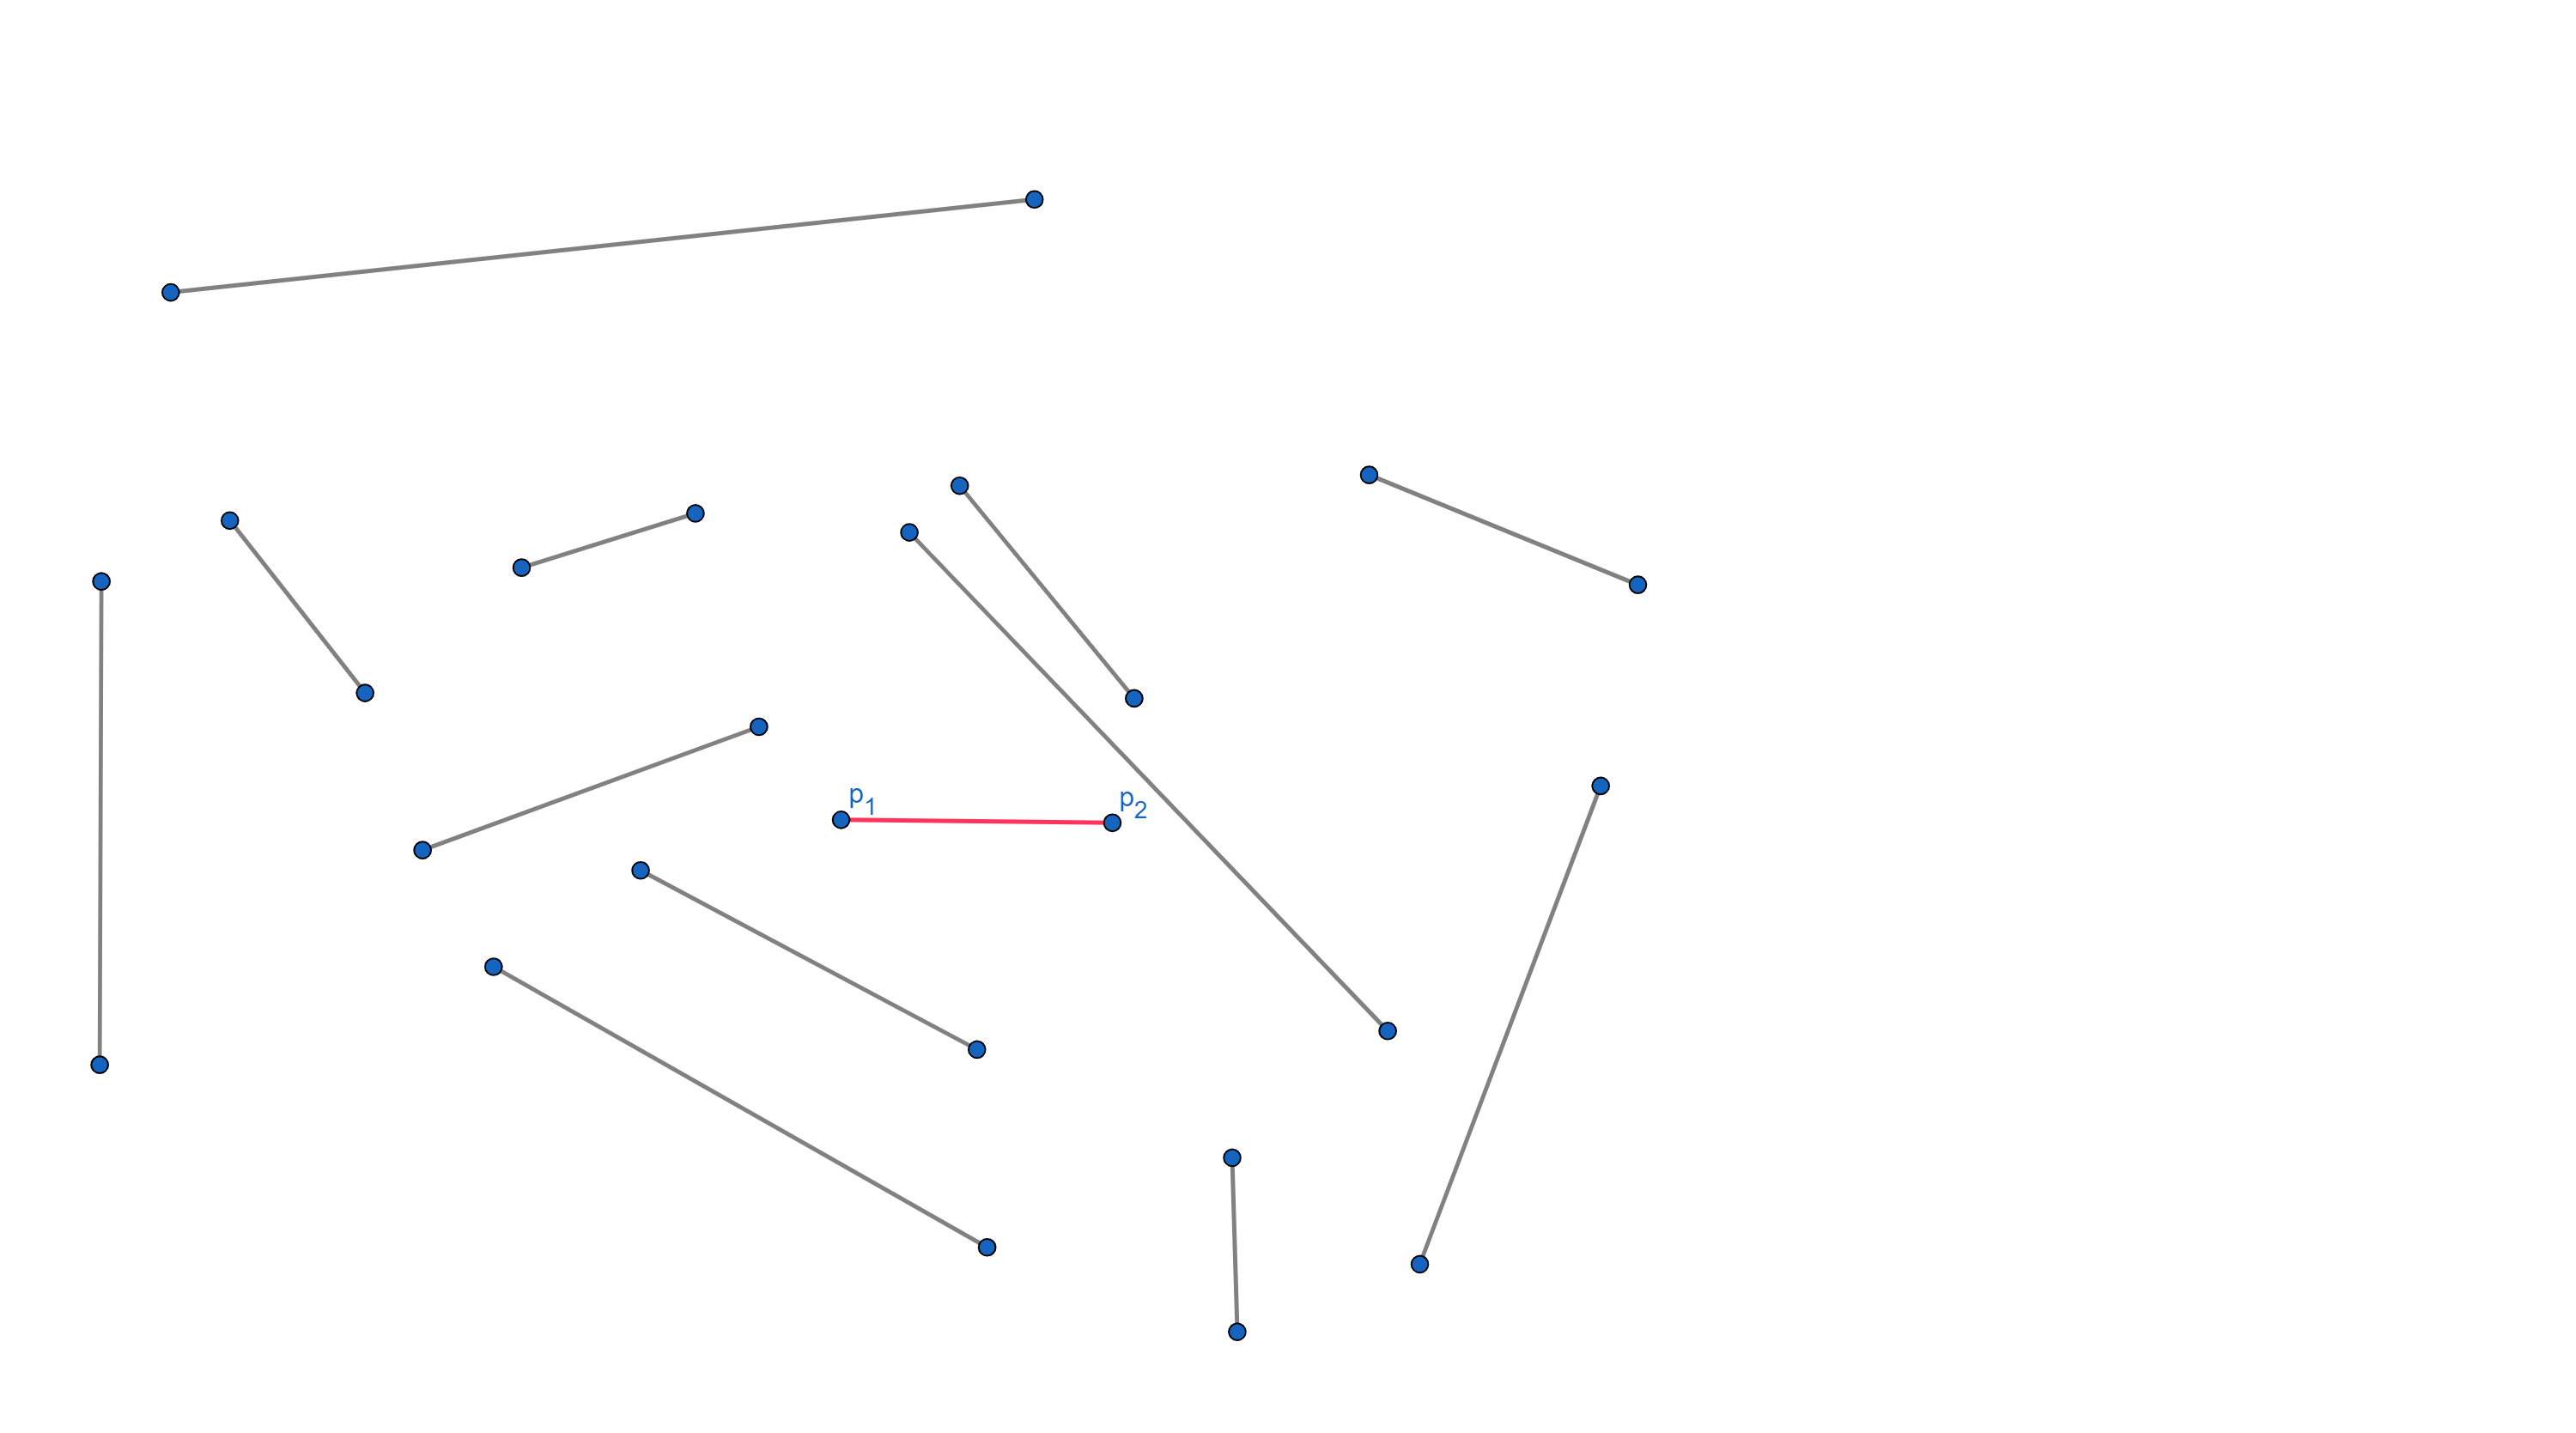
\includegraphics[width=0.5\linewidth]{segments_def.png}
\end{figure}

Множество $S$ разобьем на подмножества:

\begin{enumerate}
      \item Обе точки отрезка лежат слева от прямой, проведенной 
            через $p_1 p_2$. Обозначим $S_1$, концы -- $P_1$.
            \begin{figure}[H]
                  \centering
                  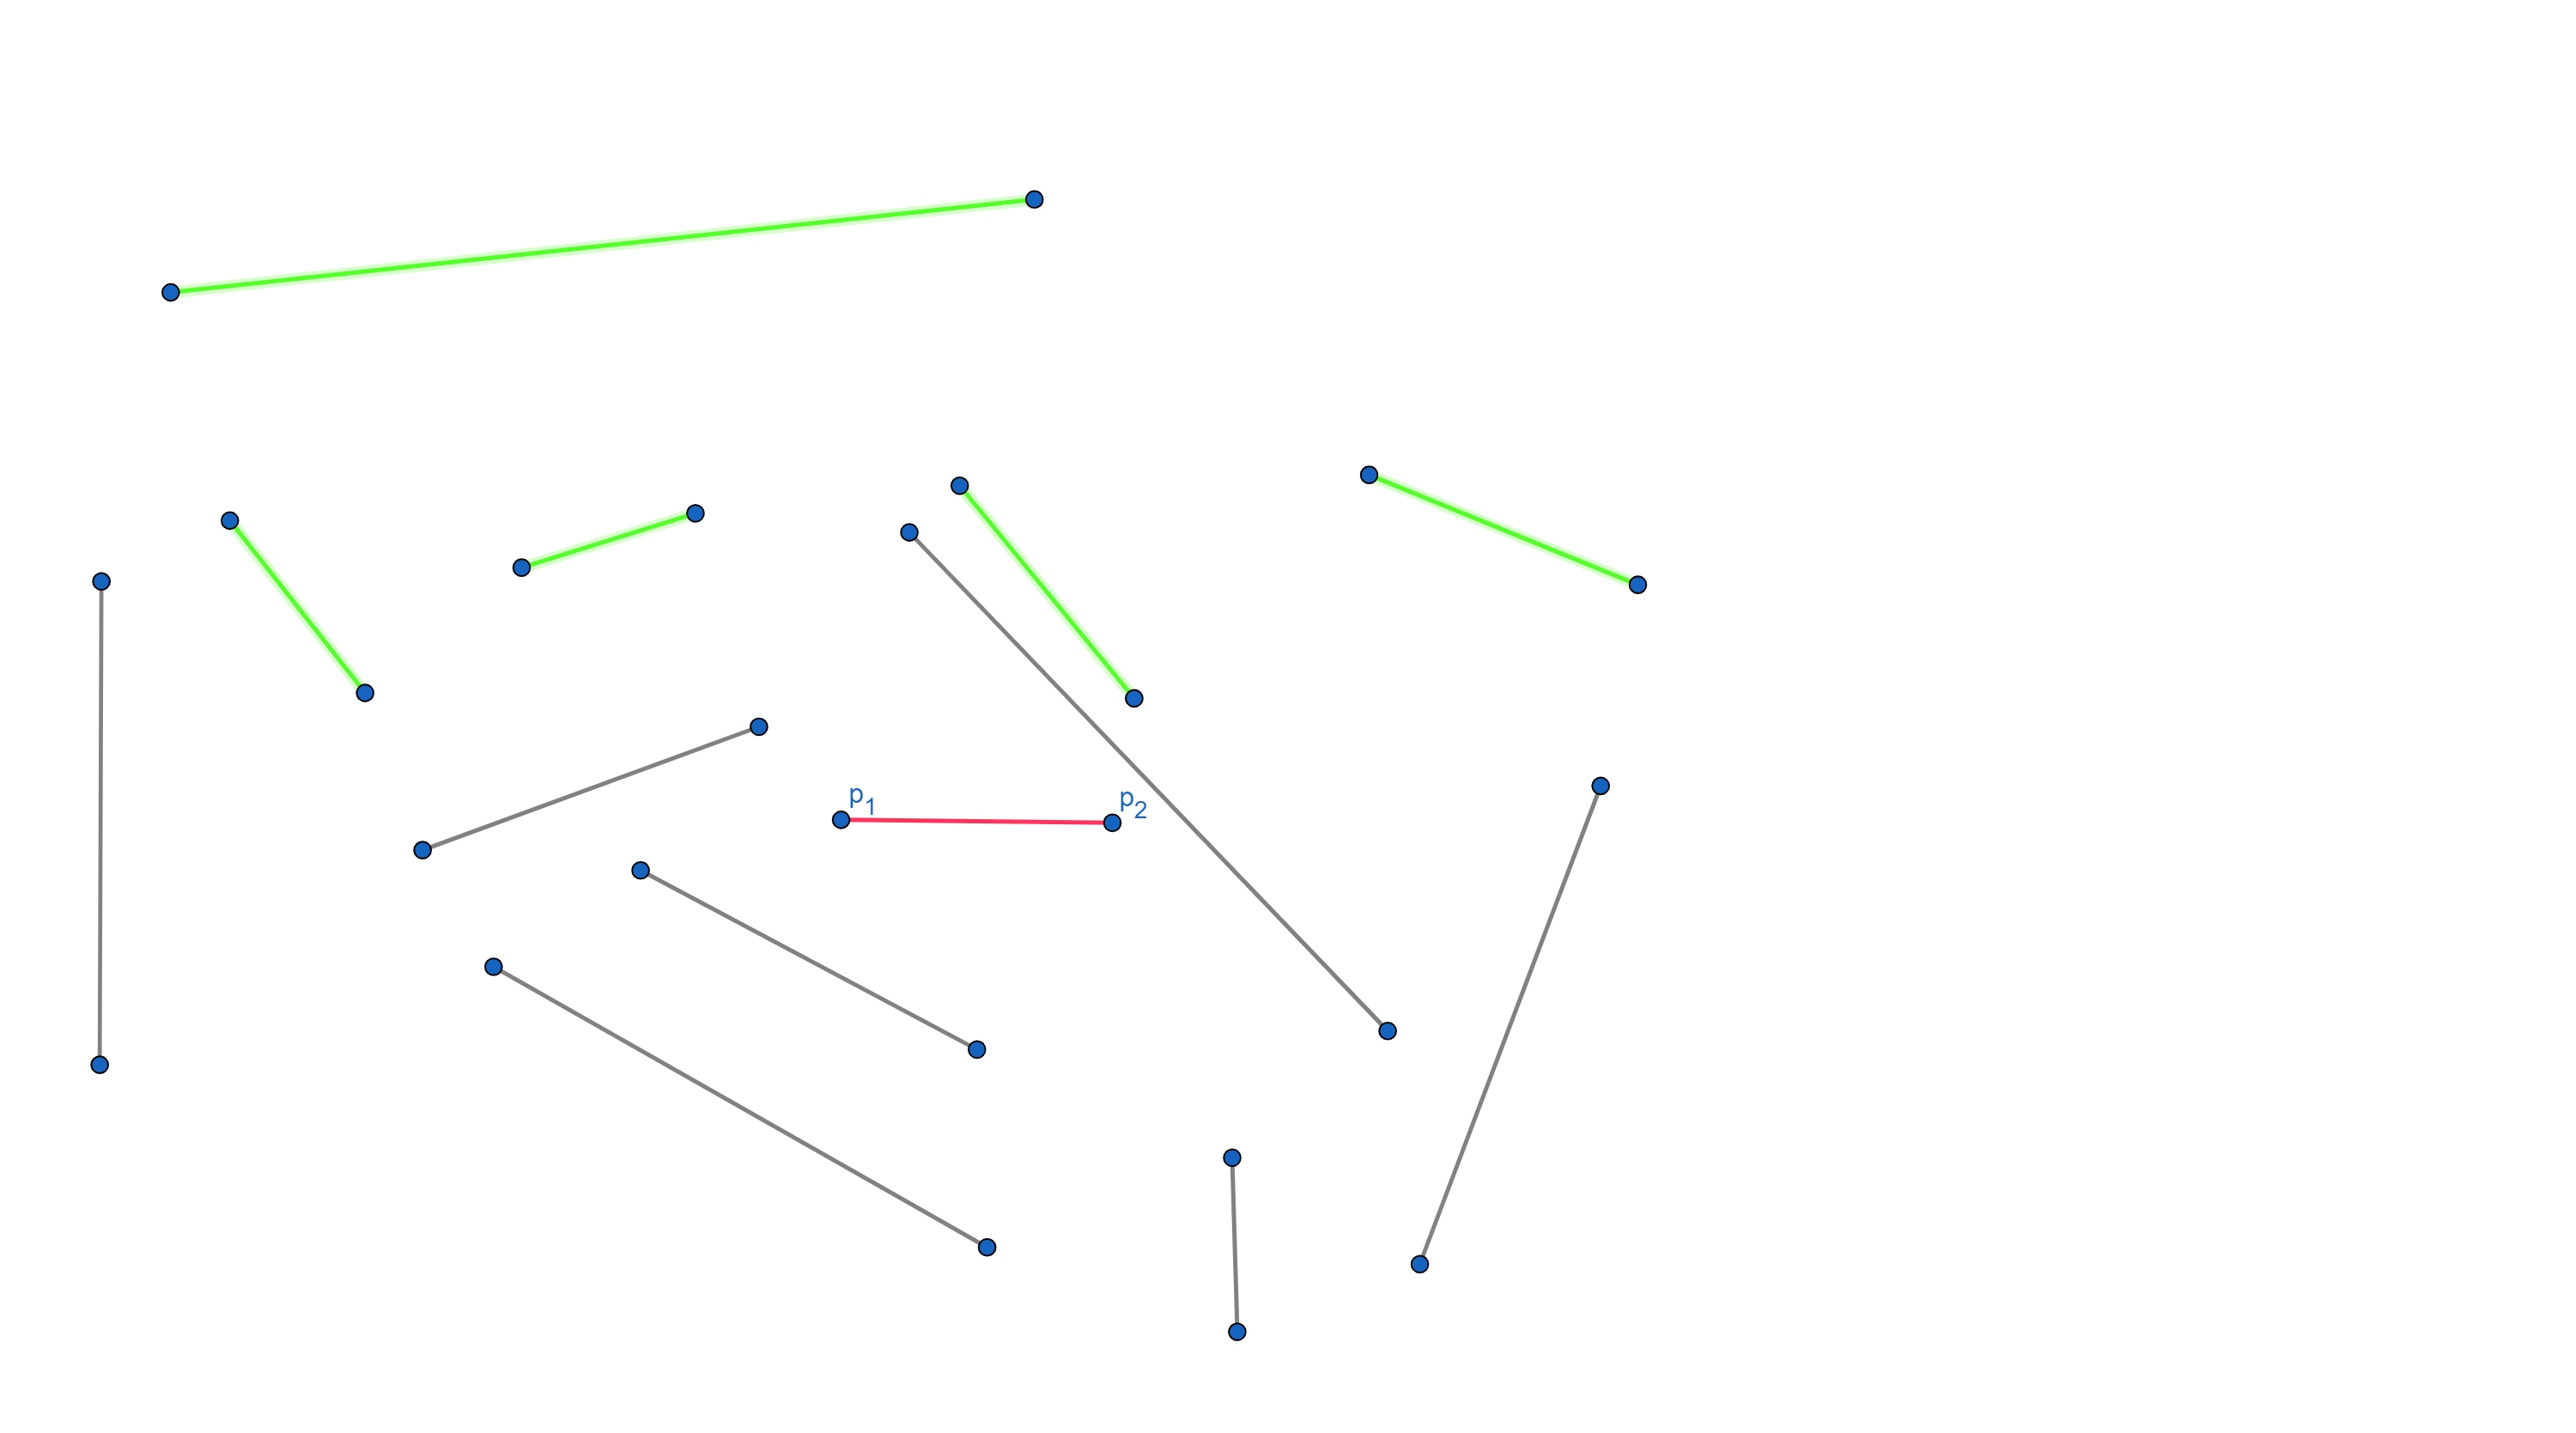
\includegraphics[width=0.5\linewidth]{segment_1.png}
            \end{figure}
      \item Обе точки отрезка лежат справа от прямой, проведенной 
            через $p_1 p_2$. Обозначим $S_2$, концы -- $P_2$.
            \begin{figure}[H]
                  \centering
                  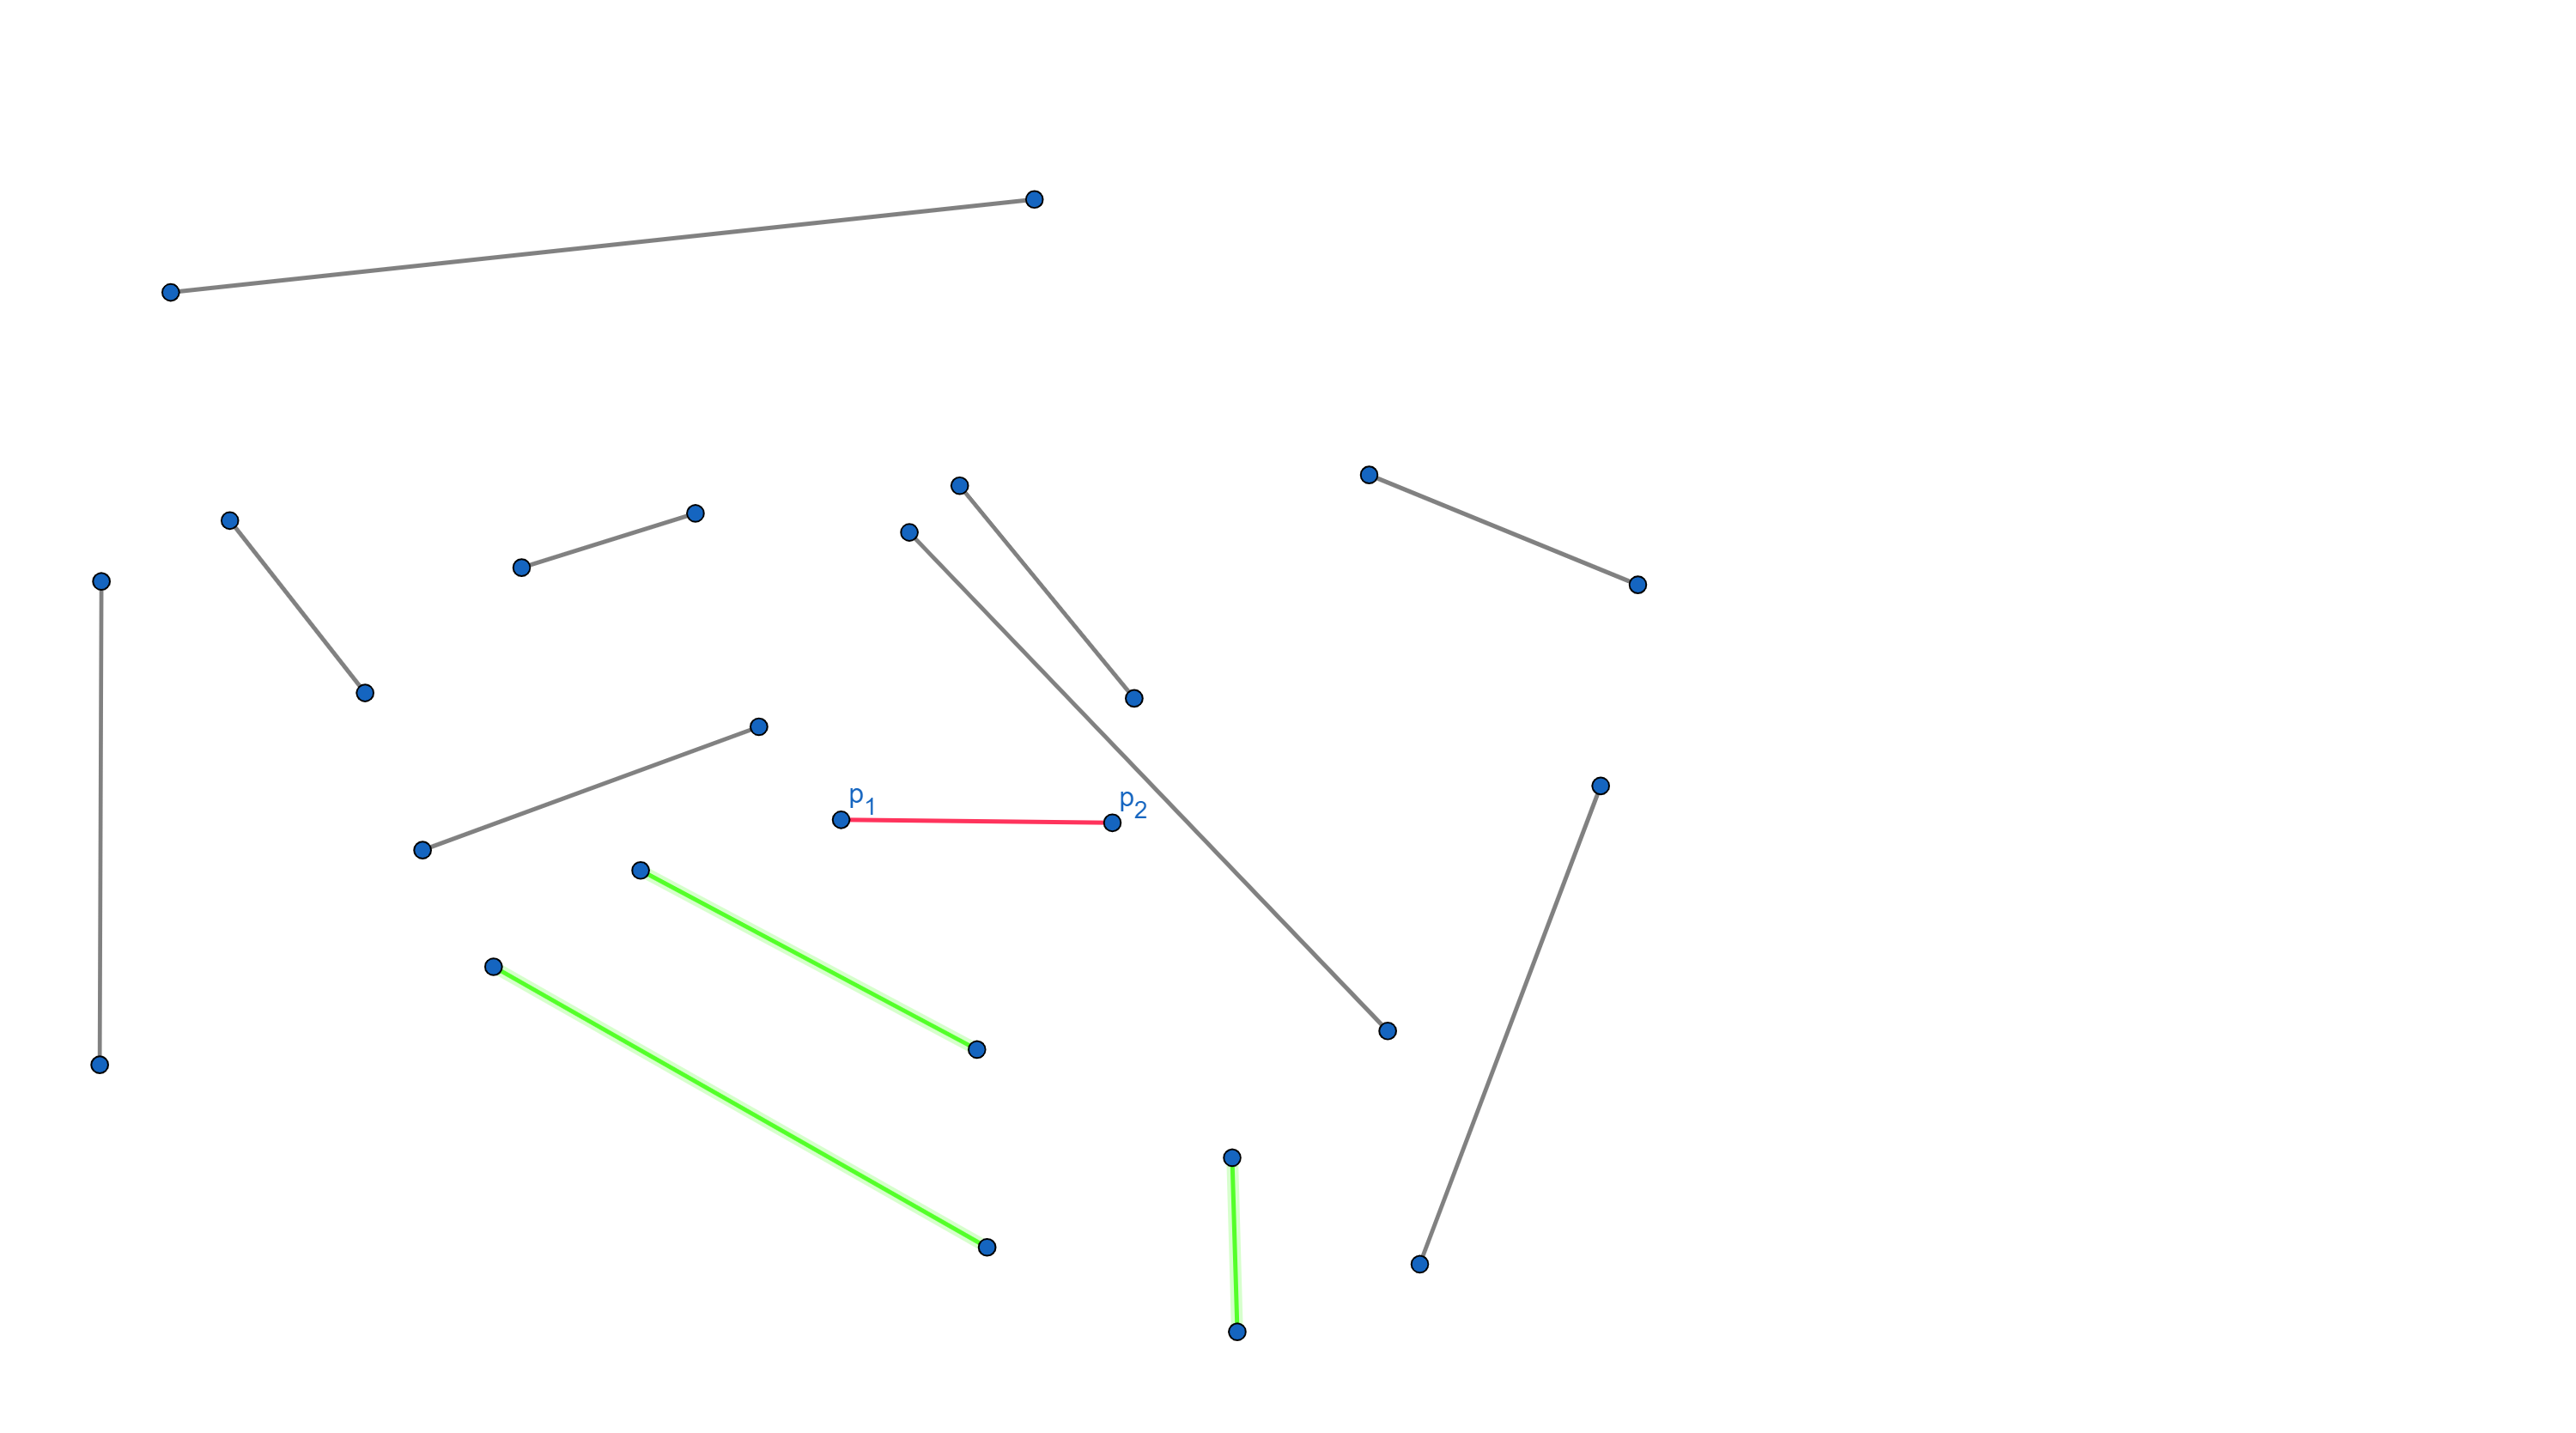
\includegraphics[width=0.5\linewidth]{segment_2.png}
            \end{figure}
      \item Точки отрезка лежат по разные стороны от прямой, 
            проведенной через $p_1 p_2$. Отрезок пересекает
            данную прямую со стороны точки $p_1$. 
            Обозначим $S_3$, концы -- $P_3$.
            \begin{figure}[H]
                  \centering
                  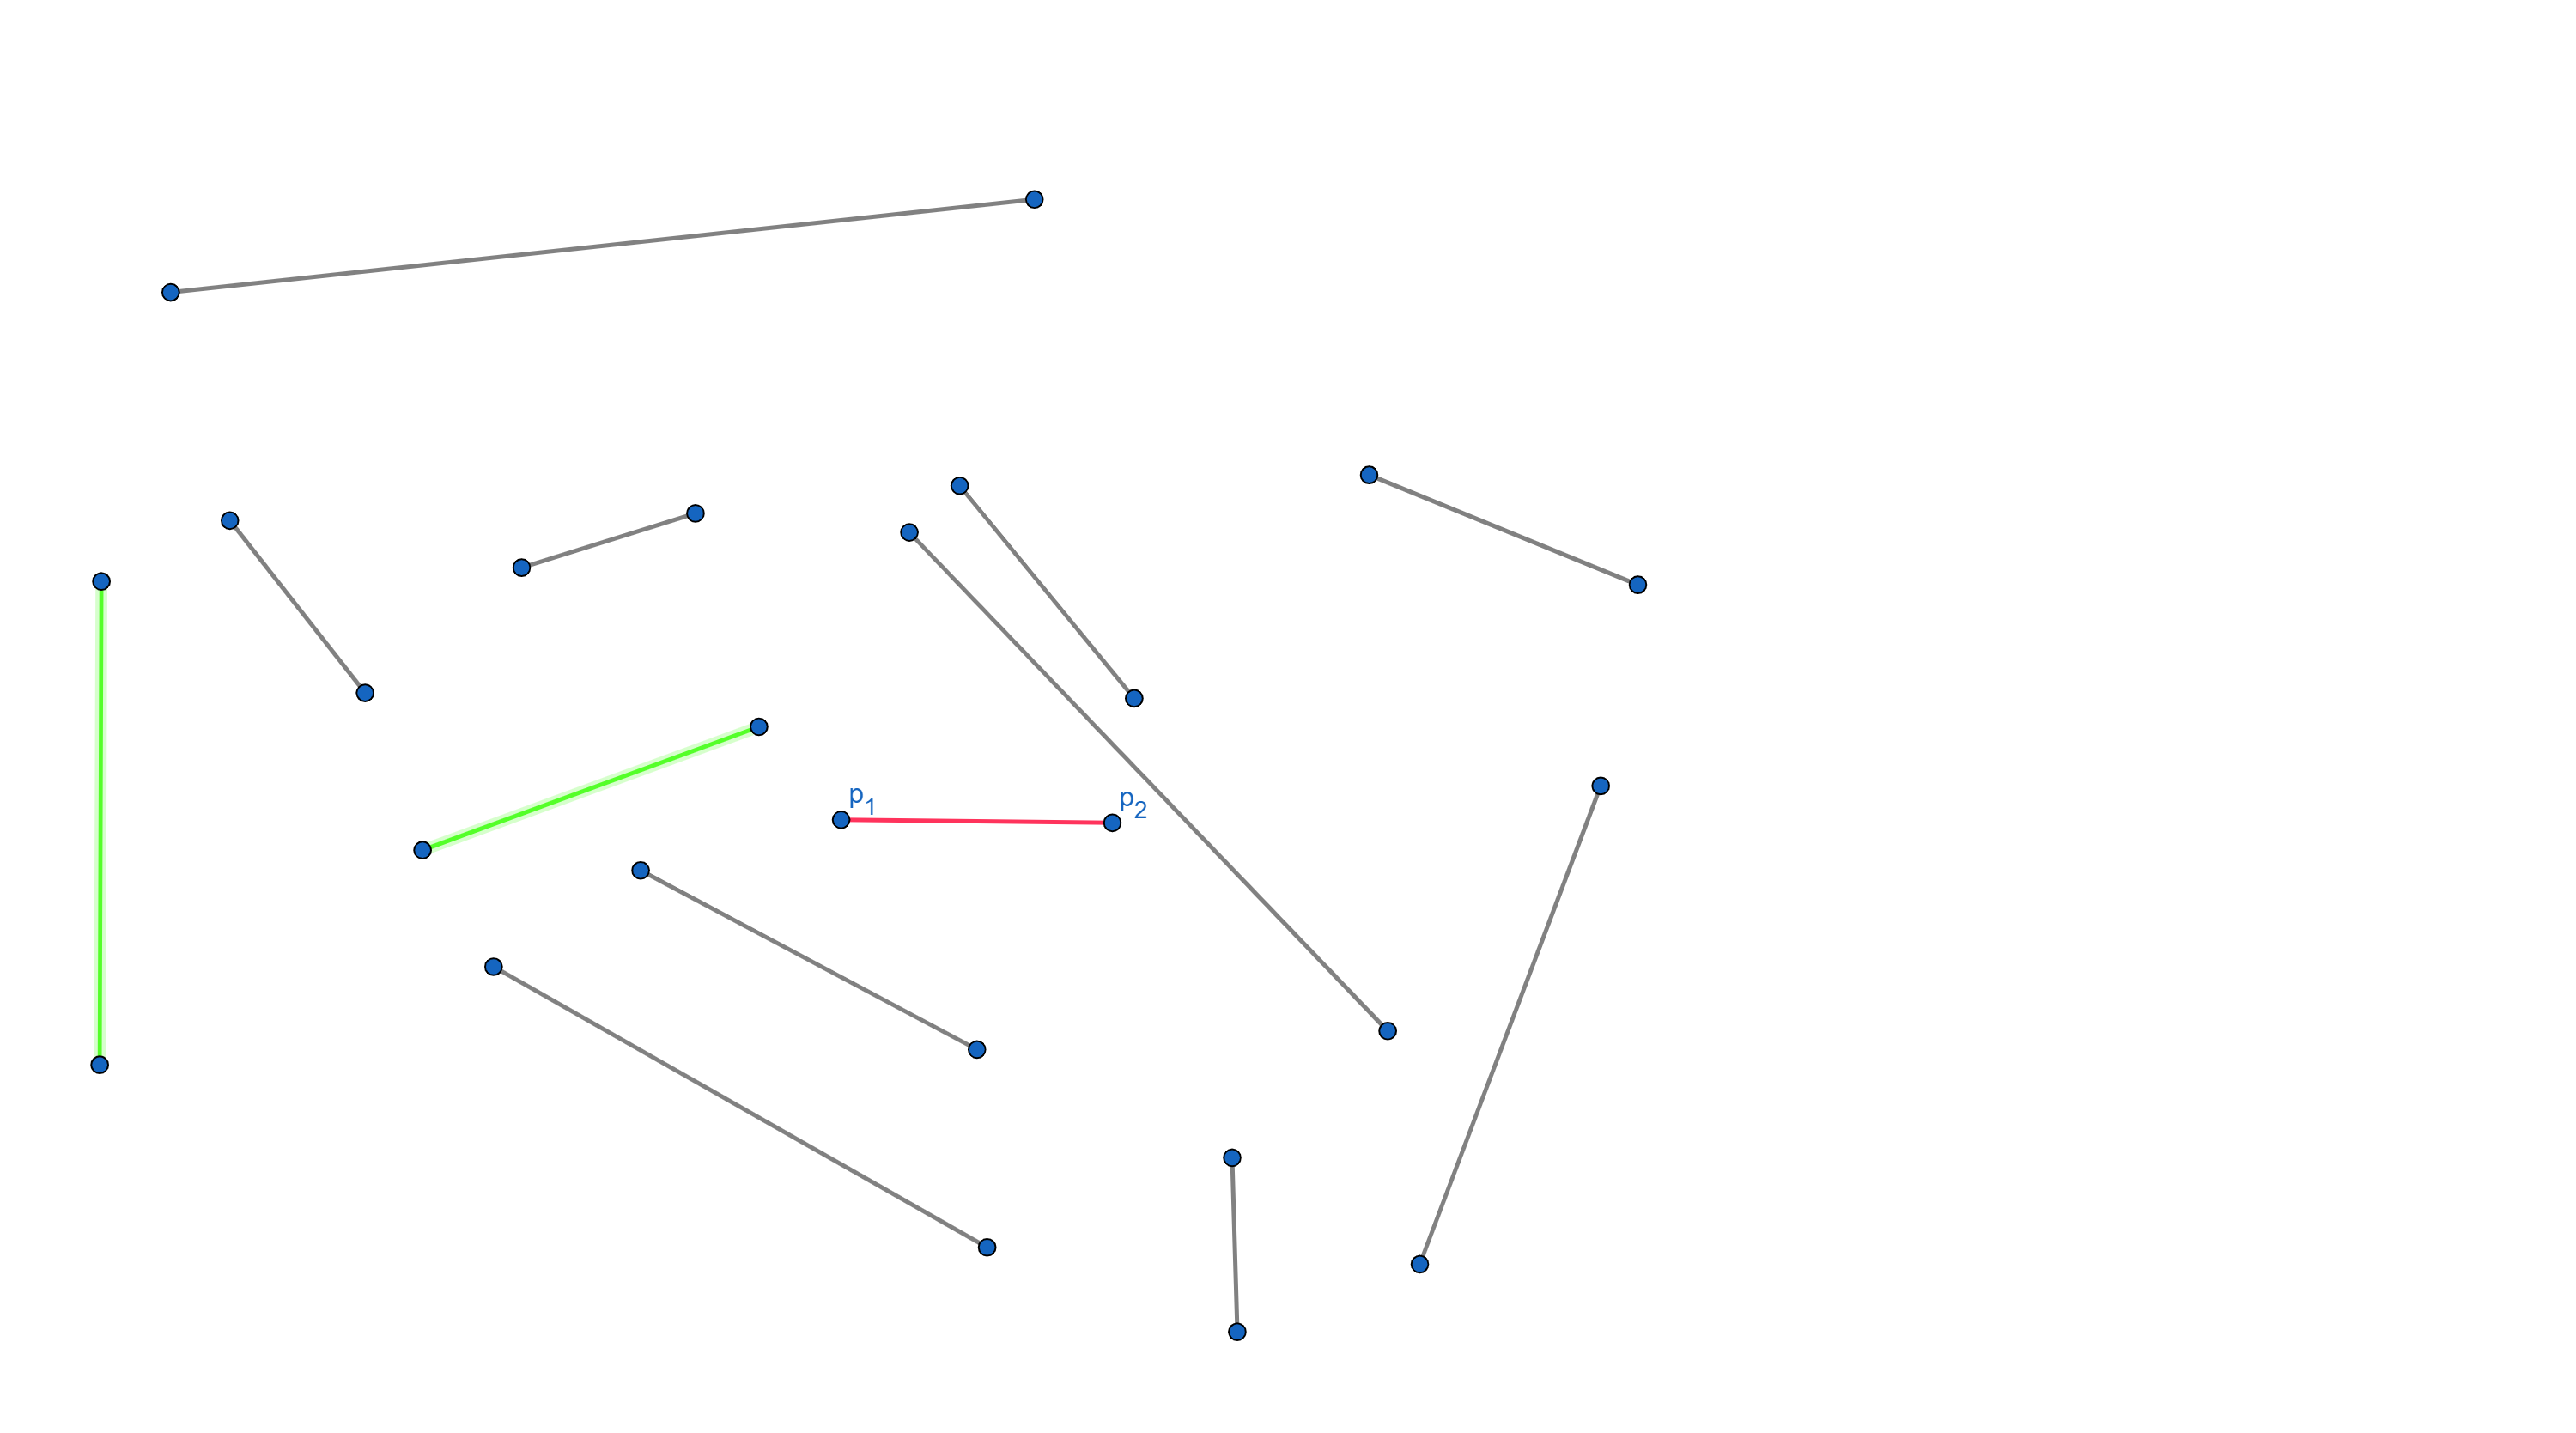
\includegraphics[width=0.5\linewidth]{segment_3.png}
            \end{figure}
      \item Точки отрезка лежат по разные стороны от прямой, 
            проведенной через $p_1 p_2$. Отрезок пересекает
            данную прямую со стороны точки $p_2$.
            Обозначим $S_4$, концы -- $P_4$.
            \begin{figure}[H]
                  \centering
                  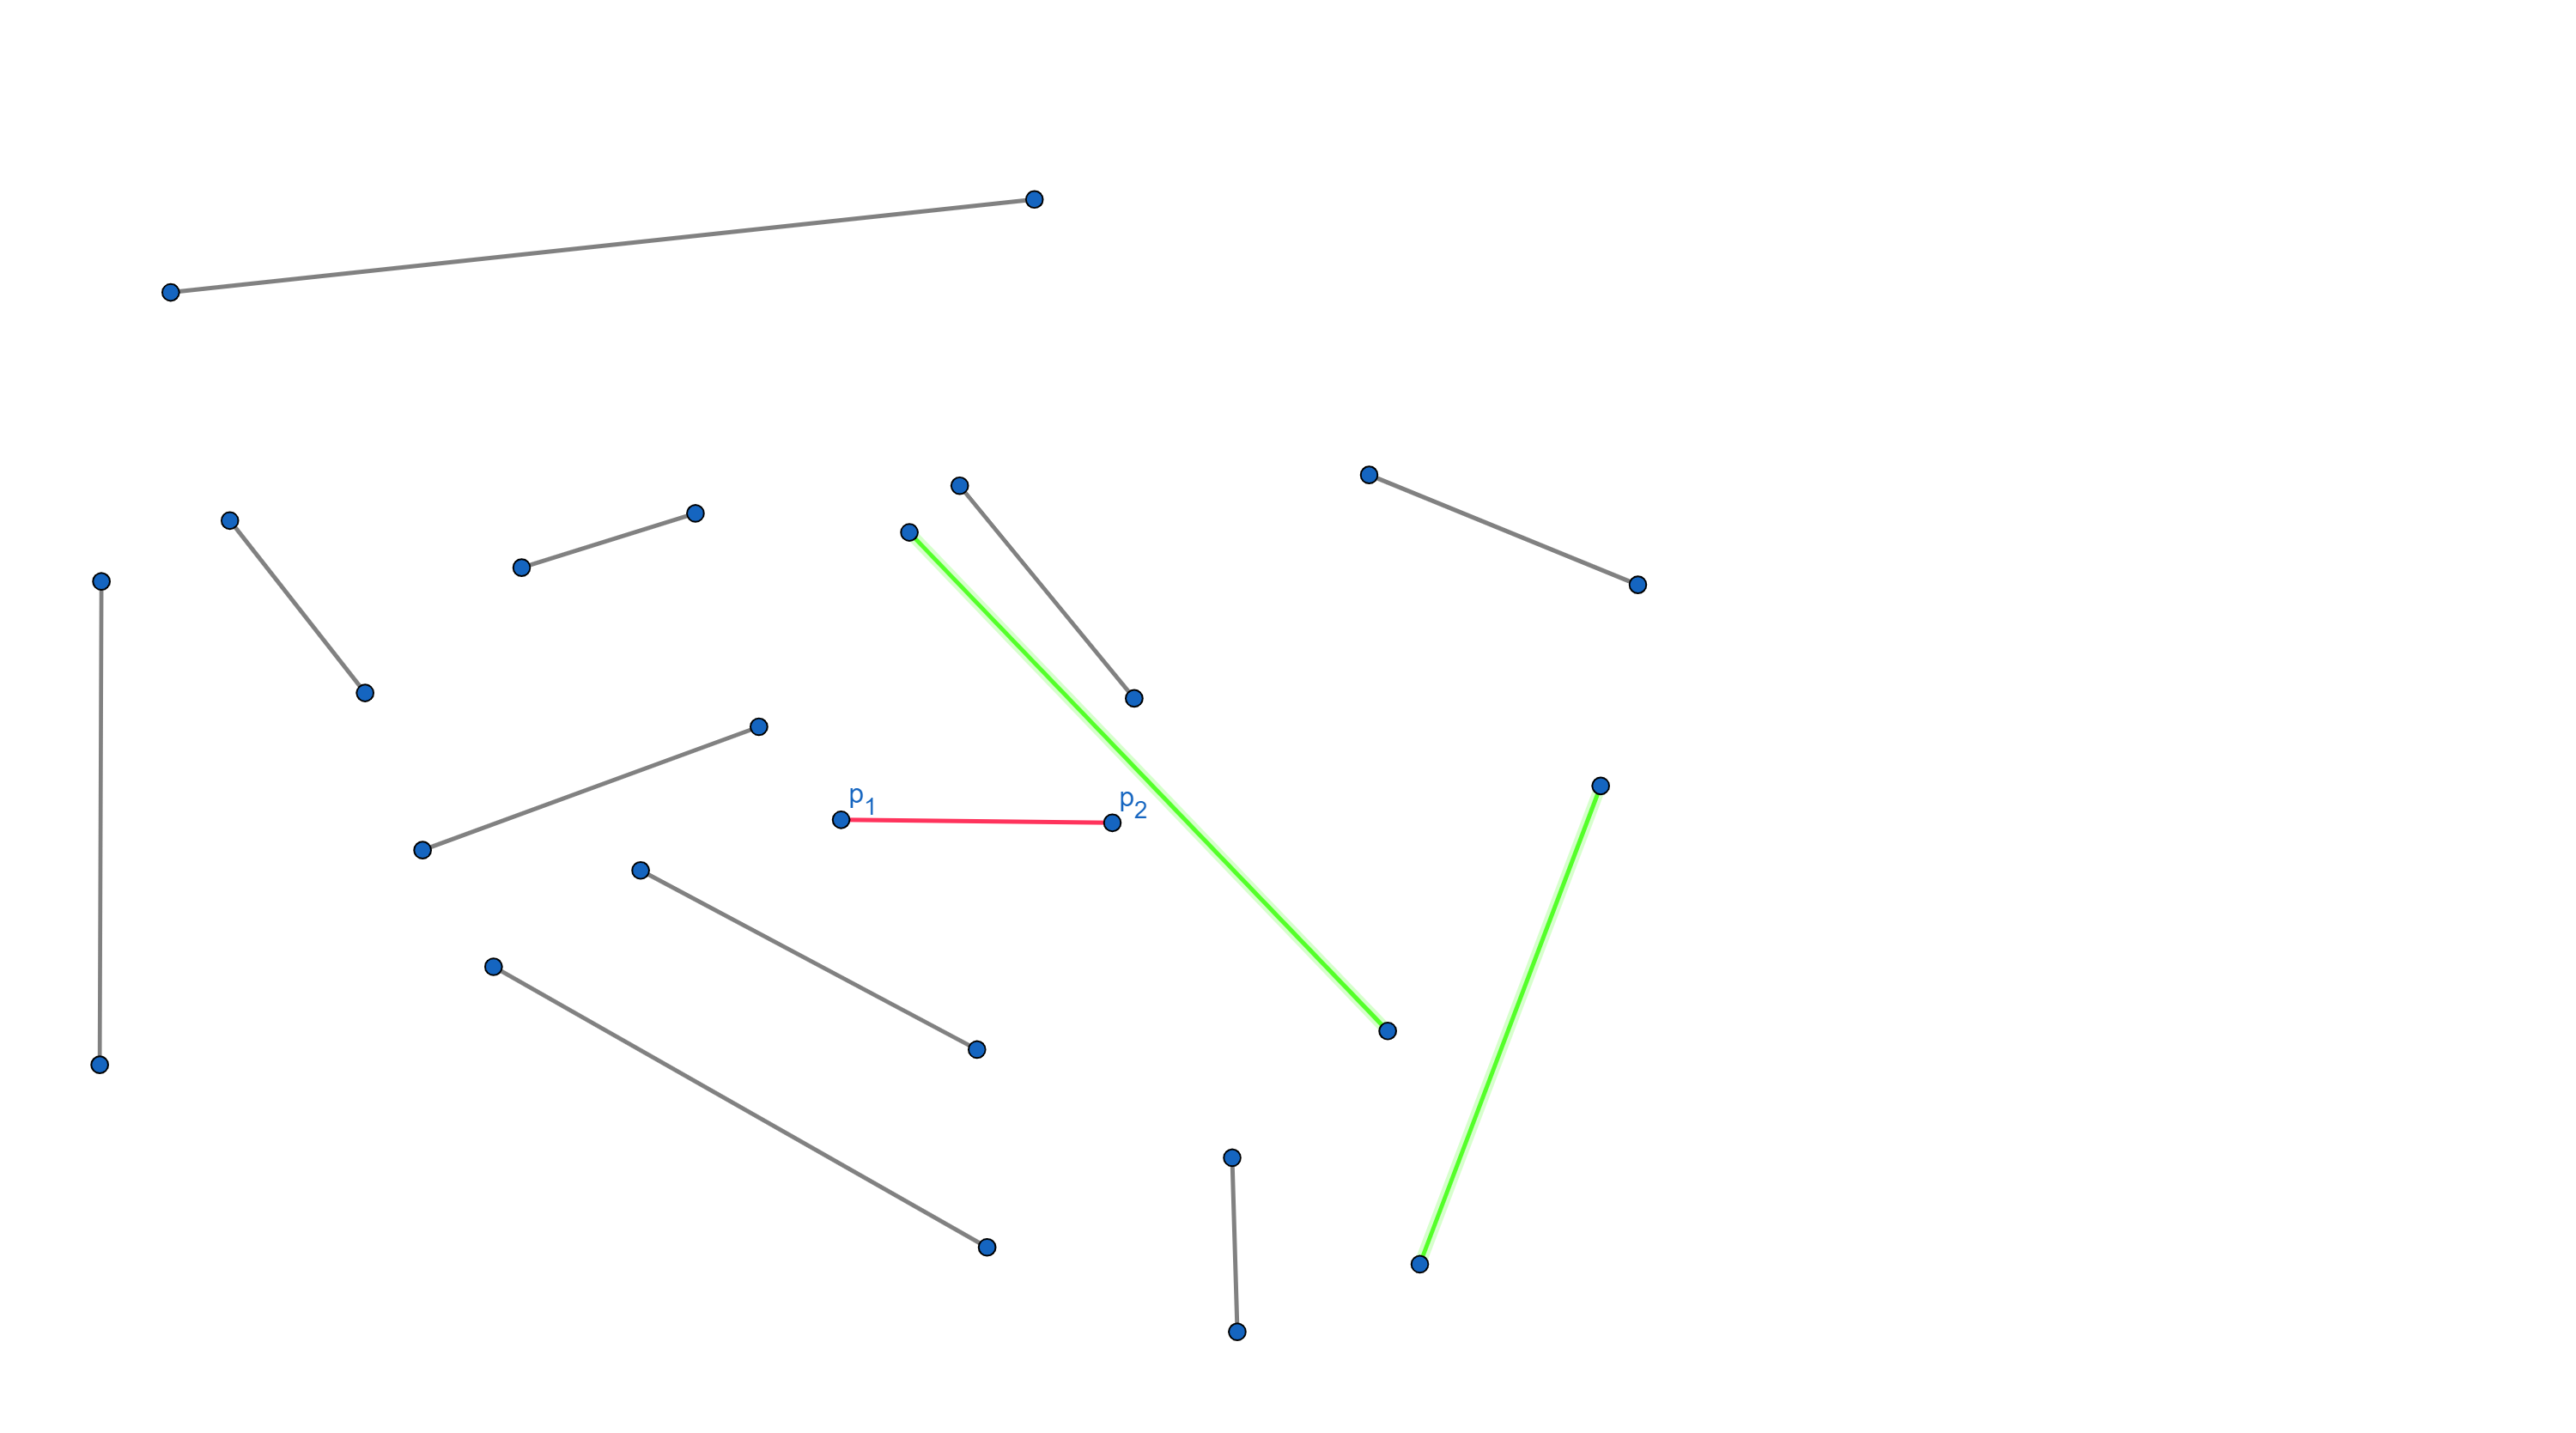
\includegraphics[width=0.5\linewidth]{segment_4.png}
            \end{figure}
            Любые другие прямые пересекали бы $p_1 p_2$.
\end{enumerate}

Рассмотрим отрезок $s_1 \in S_1$:

Определение: назовем точку $q_1 \in s_1$ левой относительно $s$,
если угол $q_1 p_1 p_2$ максимален по всем $q \in s_1$.

Определение: назовем точку $q_2 \in s_1$ правой относительно $s$,
если угол $q_1 p_2 p_1$ максимален по всем $q \in s_1$.

Замечание: точка отрезка может быть одновременно левой и правой.

\begin{figure}[H]
      \centering
      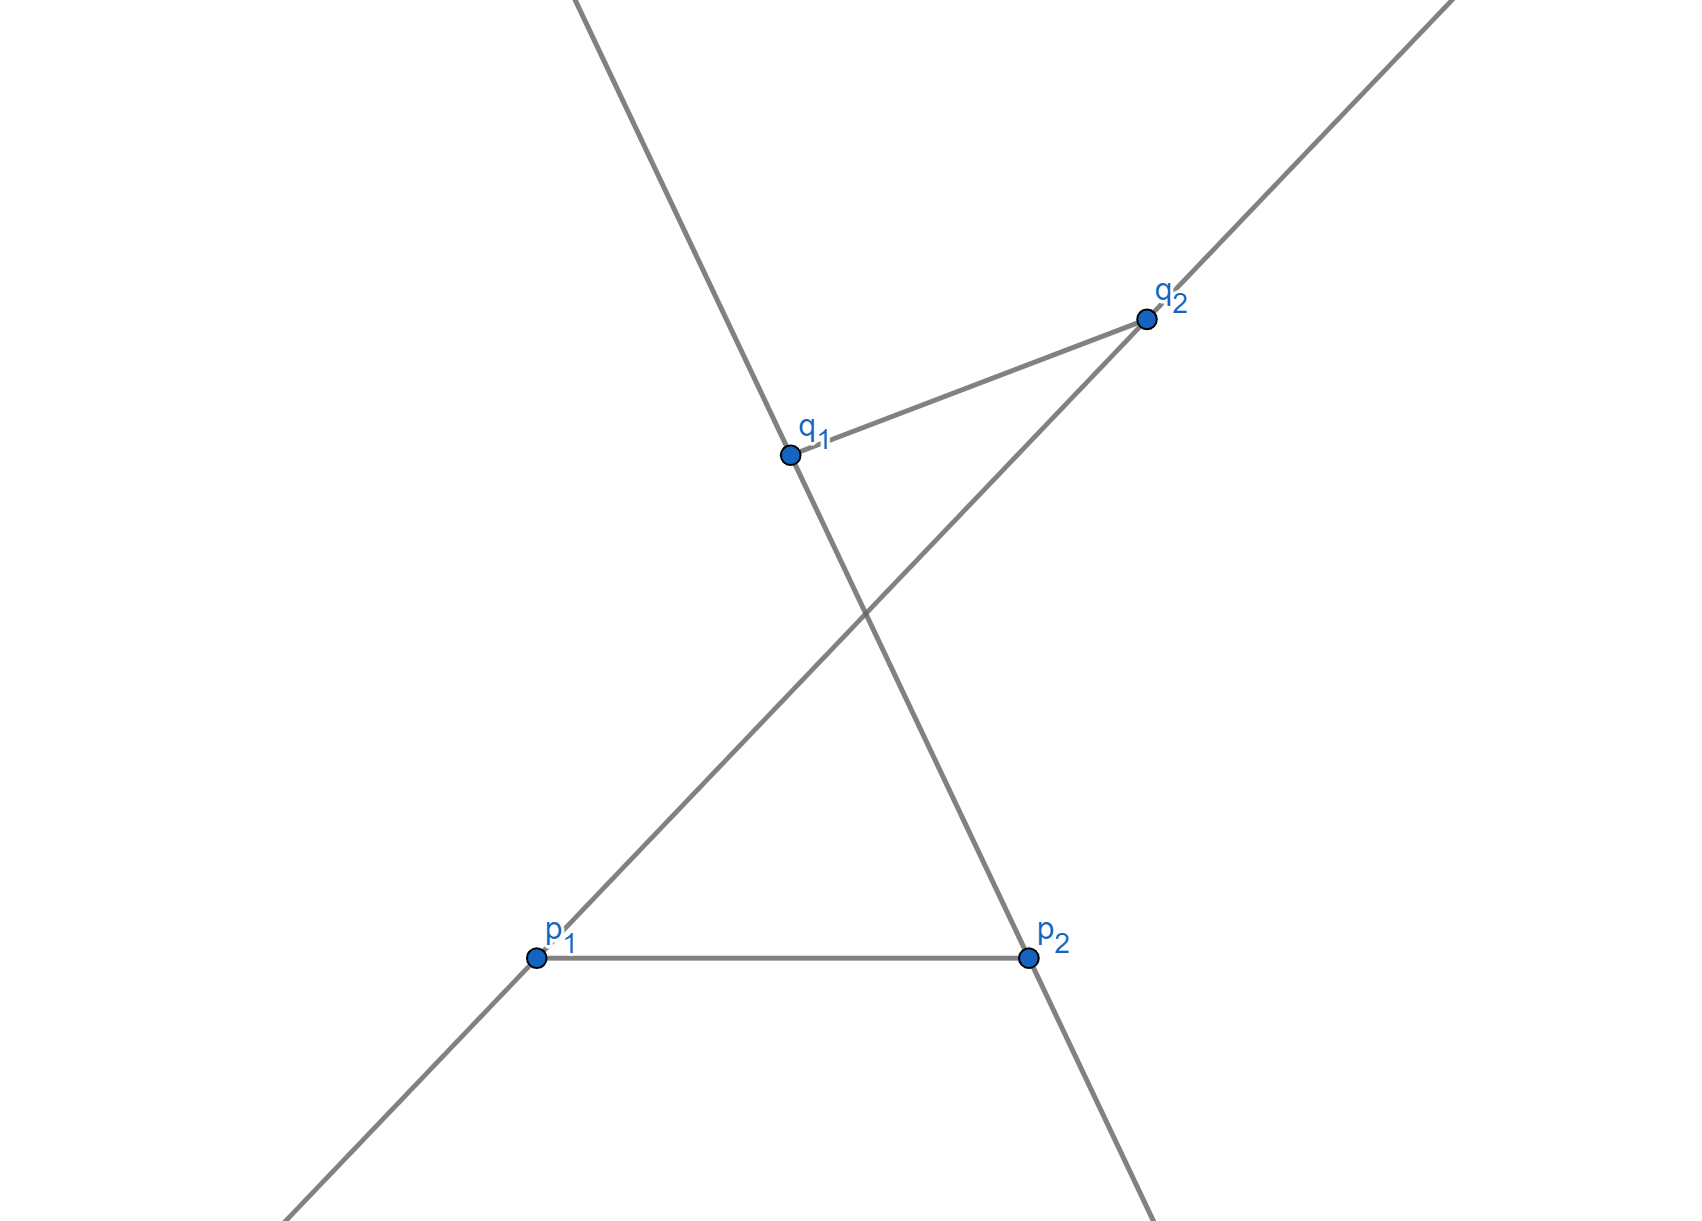
\includegraphics[width=0.5\linewidth]{one_segment_q1q2.png}
\end{figure}

Утверждение: левая и правая точки всегда являются концами отрезка.

\begin{figure}[H]
      \centering
      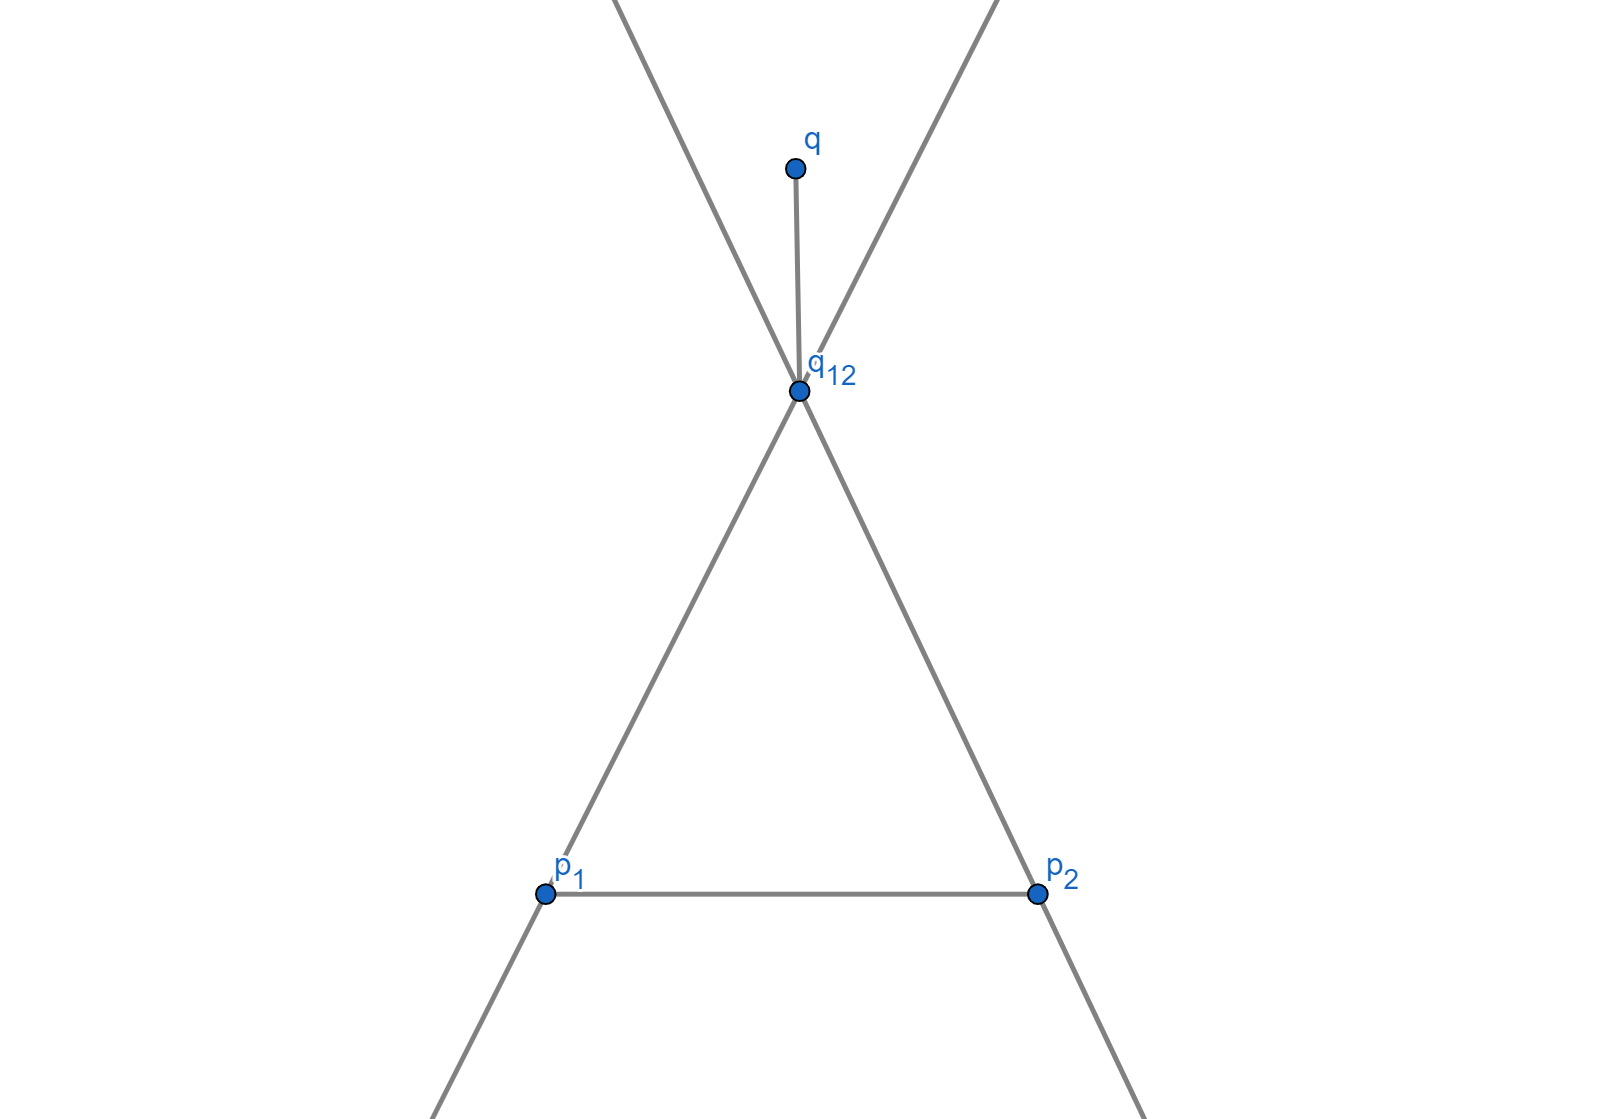
\includegraphics[width=0.5\linewidth]{one_segment_q12.png}
\end{figure}

Утверждение: нет-зона отрезка $s$ относительно $s_1 \in S_1$
лежит ниже прямой, проходящей через отрезок $s$, содержит часть
пространства, отсекаемого лучами, начинающимися из точек 
$p_1$ и $p_2$, лежащими на прямых, заданных $q_1 p_2$, $q_2 p_1$.

\begin{figure}[H]
      \centering
      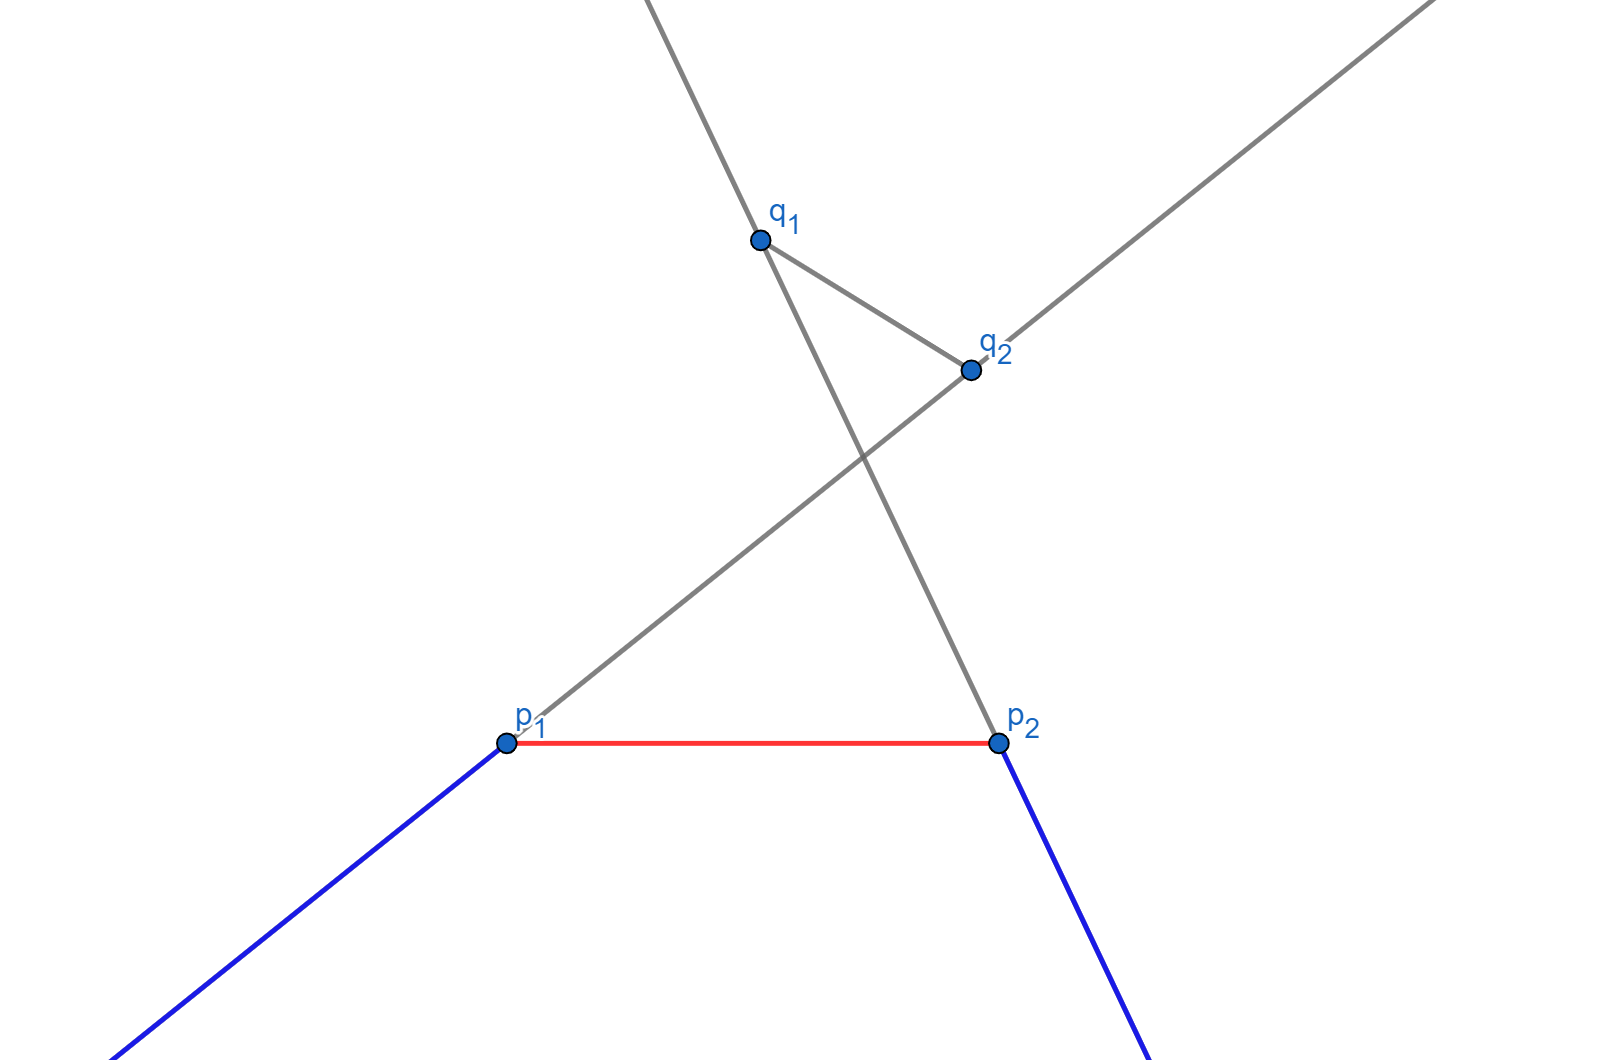
\includegraphics[width=0.5\linewidth]{no_zone_s1.png}
\end{figure}

Утверждение: нет-зона отрезка $s$ относительно $S_1$ имеет
сложность $O(n)$, где $n$ -- количество отрезков в $S_1$.

Построим множество ${S_1}'$ такое, что все содержащиеся в нем
отрезки имеют следующие свойства:

\begin{enumerate}
      \item $s_1 \in S_1$
      \item сущетвует подмножество декартовой плоскости,
            отсеченное параллельными прямыми $l_1$, $l_2$,
            проходящими через точки $p_1$ и $p_2$ соответсвенно,
            содержащее минимум одну из правой и левой точек
            каждого отрезка.
\end{enumerate}

Утверждение: нет-зона отрезка $s$ относительно ${S_1}'$ имеет
сложность $O(1)$.

\begin{figure}[H]
      \centering
      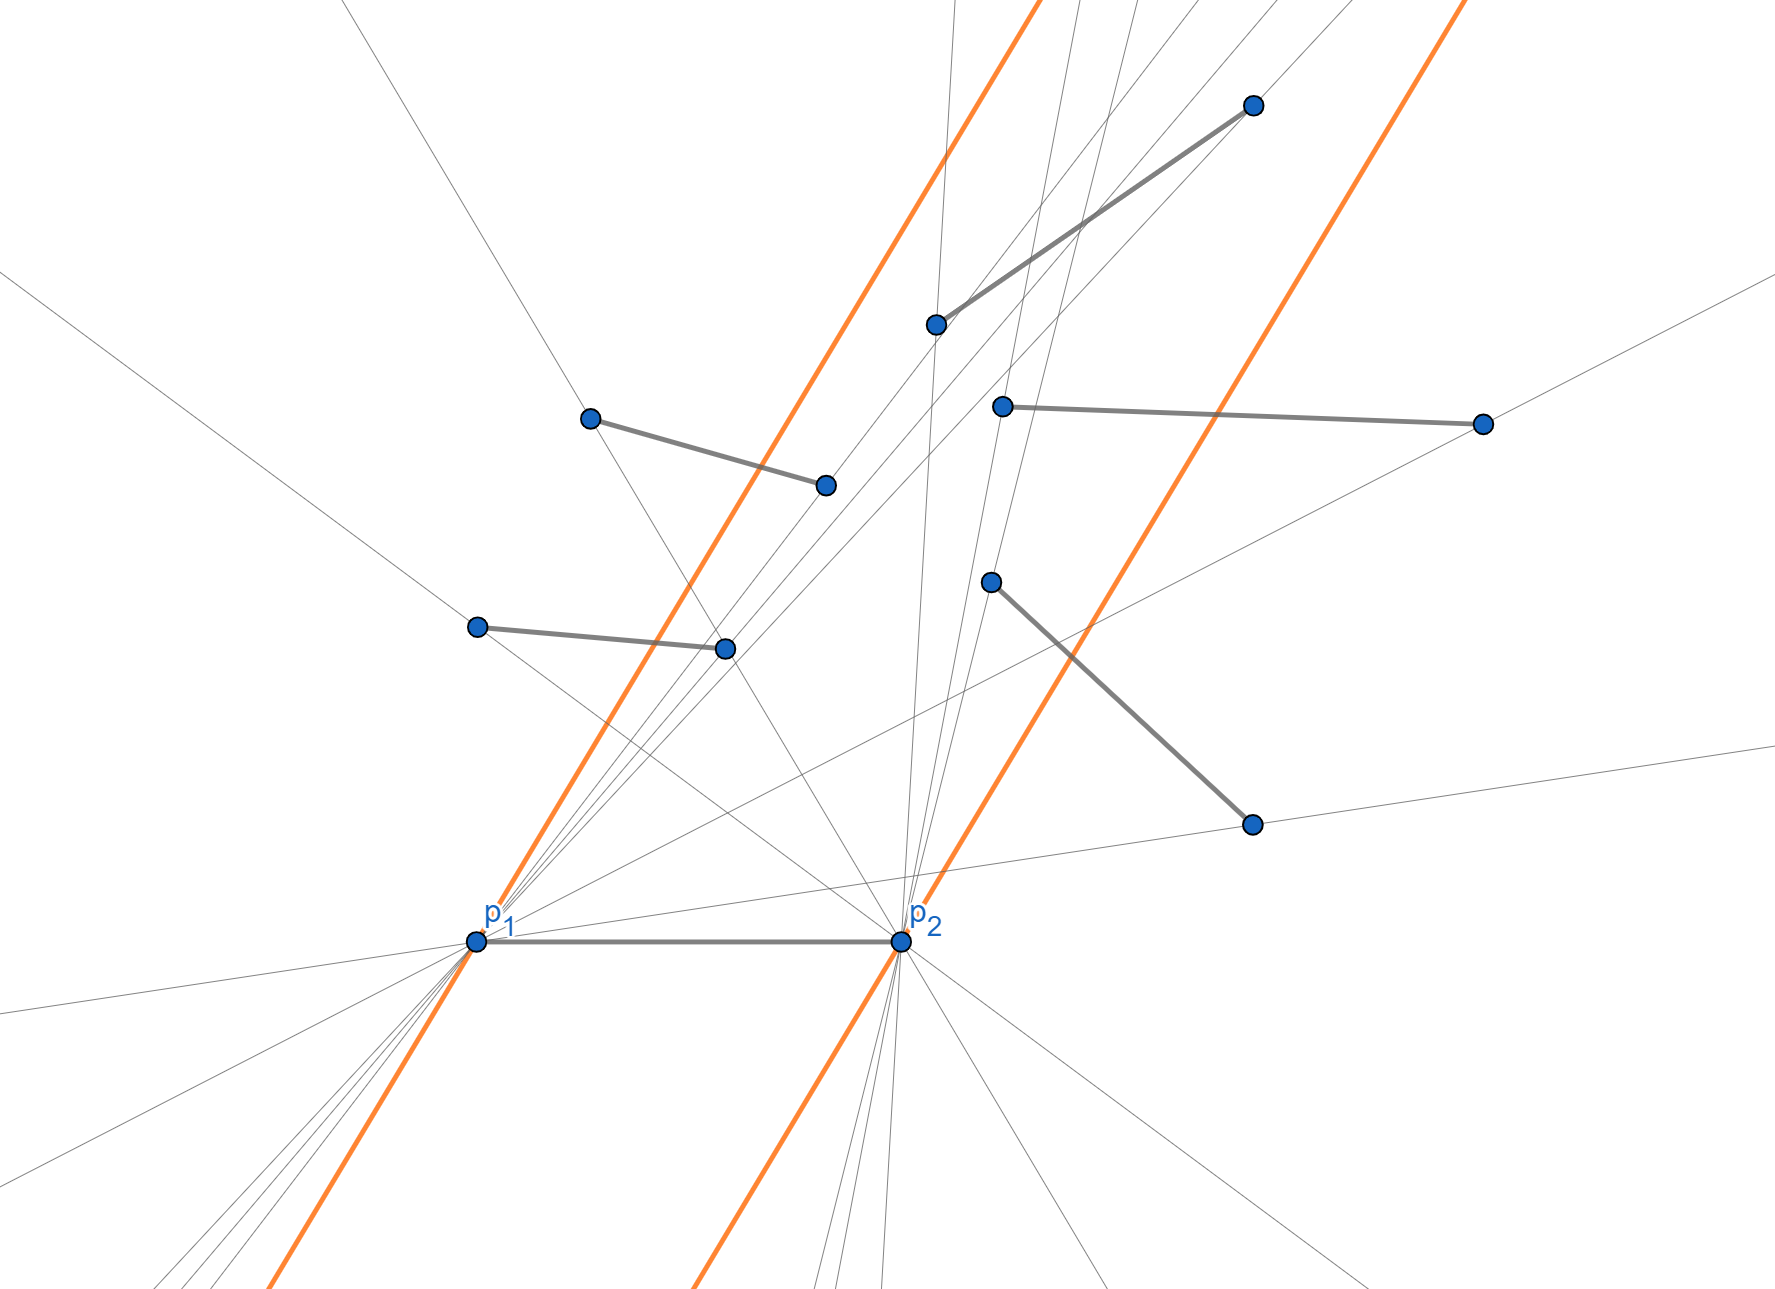
\includegraphics[width=0.5\linewidth]{no_zone_S1_.png}
\end{figure}

Существование хотя бы одного отрезка в $S_1$ порождает
одну область <<нет-зоны>>. В зависимости от взаимного
расположения отрезков ее сложность - $O(n)$.

\begin{figure}[H]
      \centering
      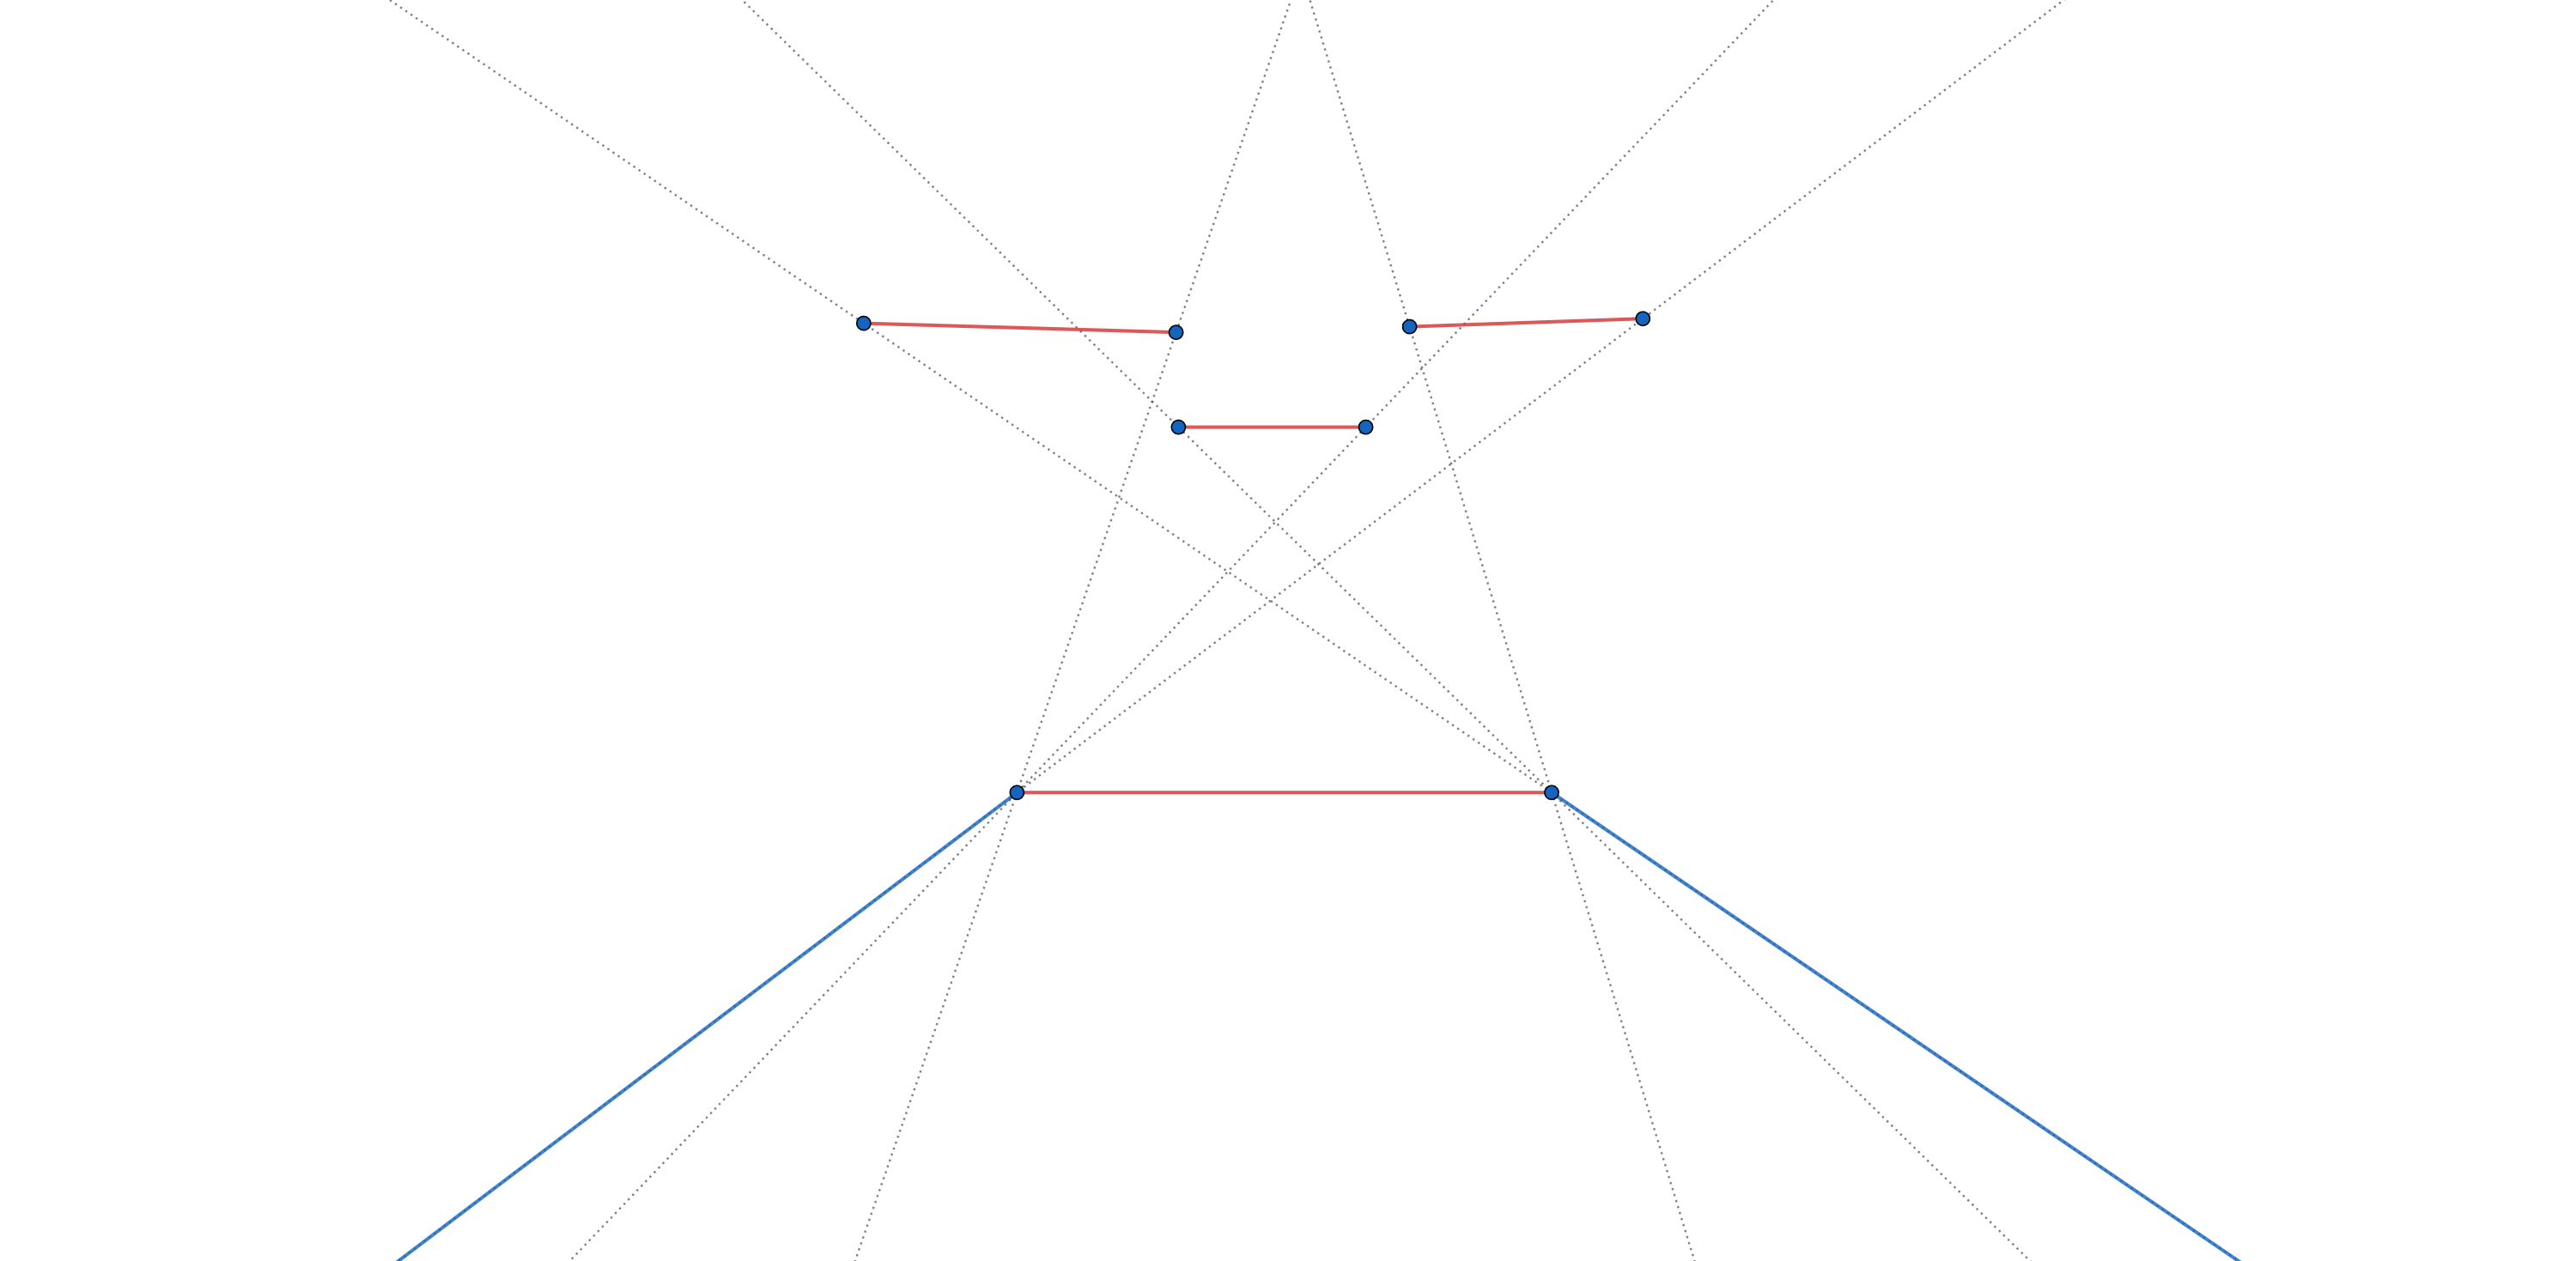
\includegraphics[width=0.5\linewidth]{no_zone_S1_simple.png}
\end{figure}

\begin{figure}[H]
      \centering
      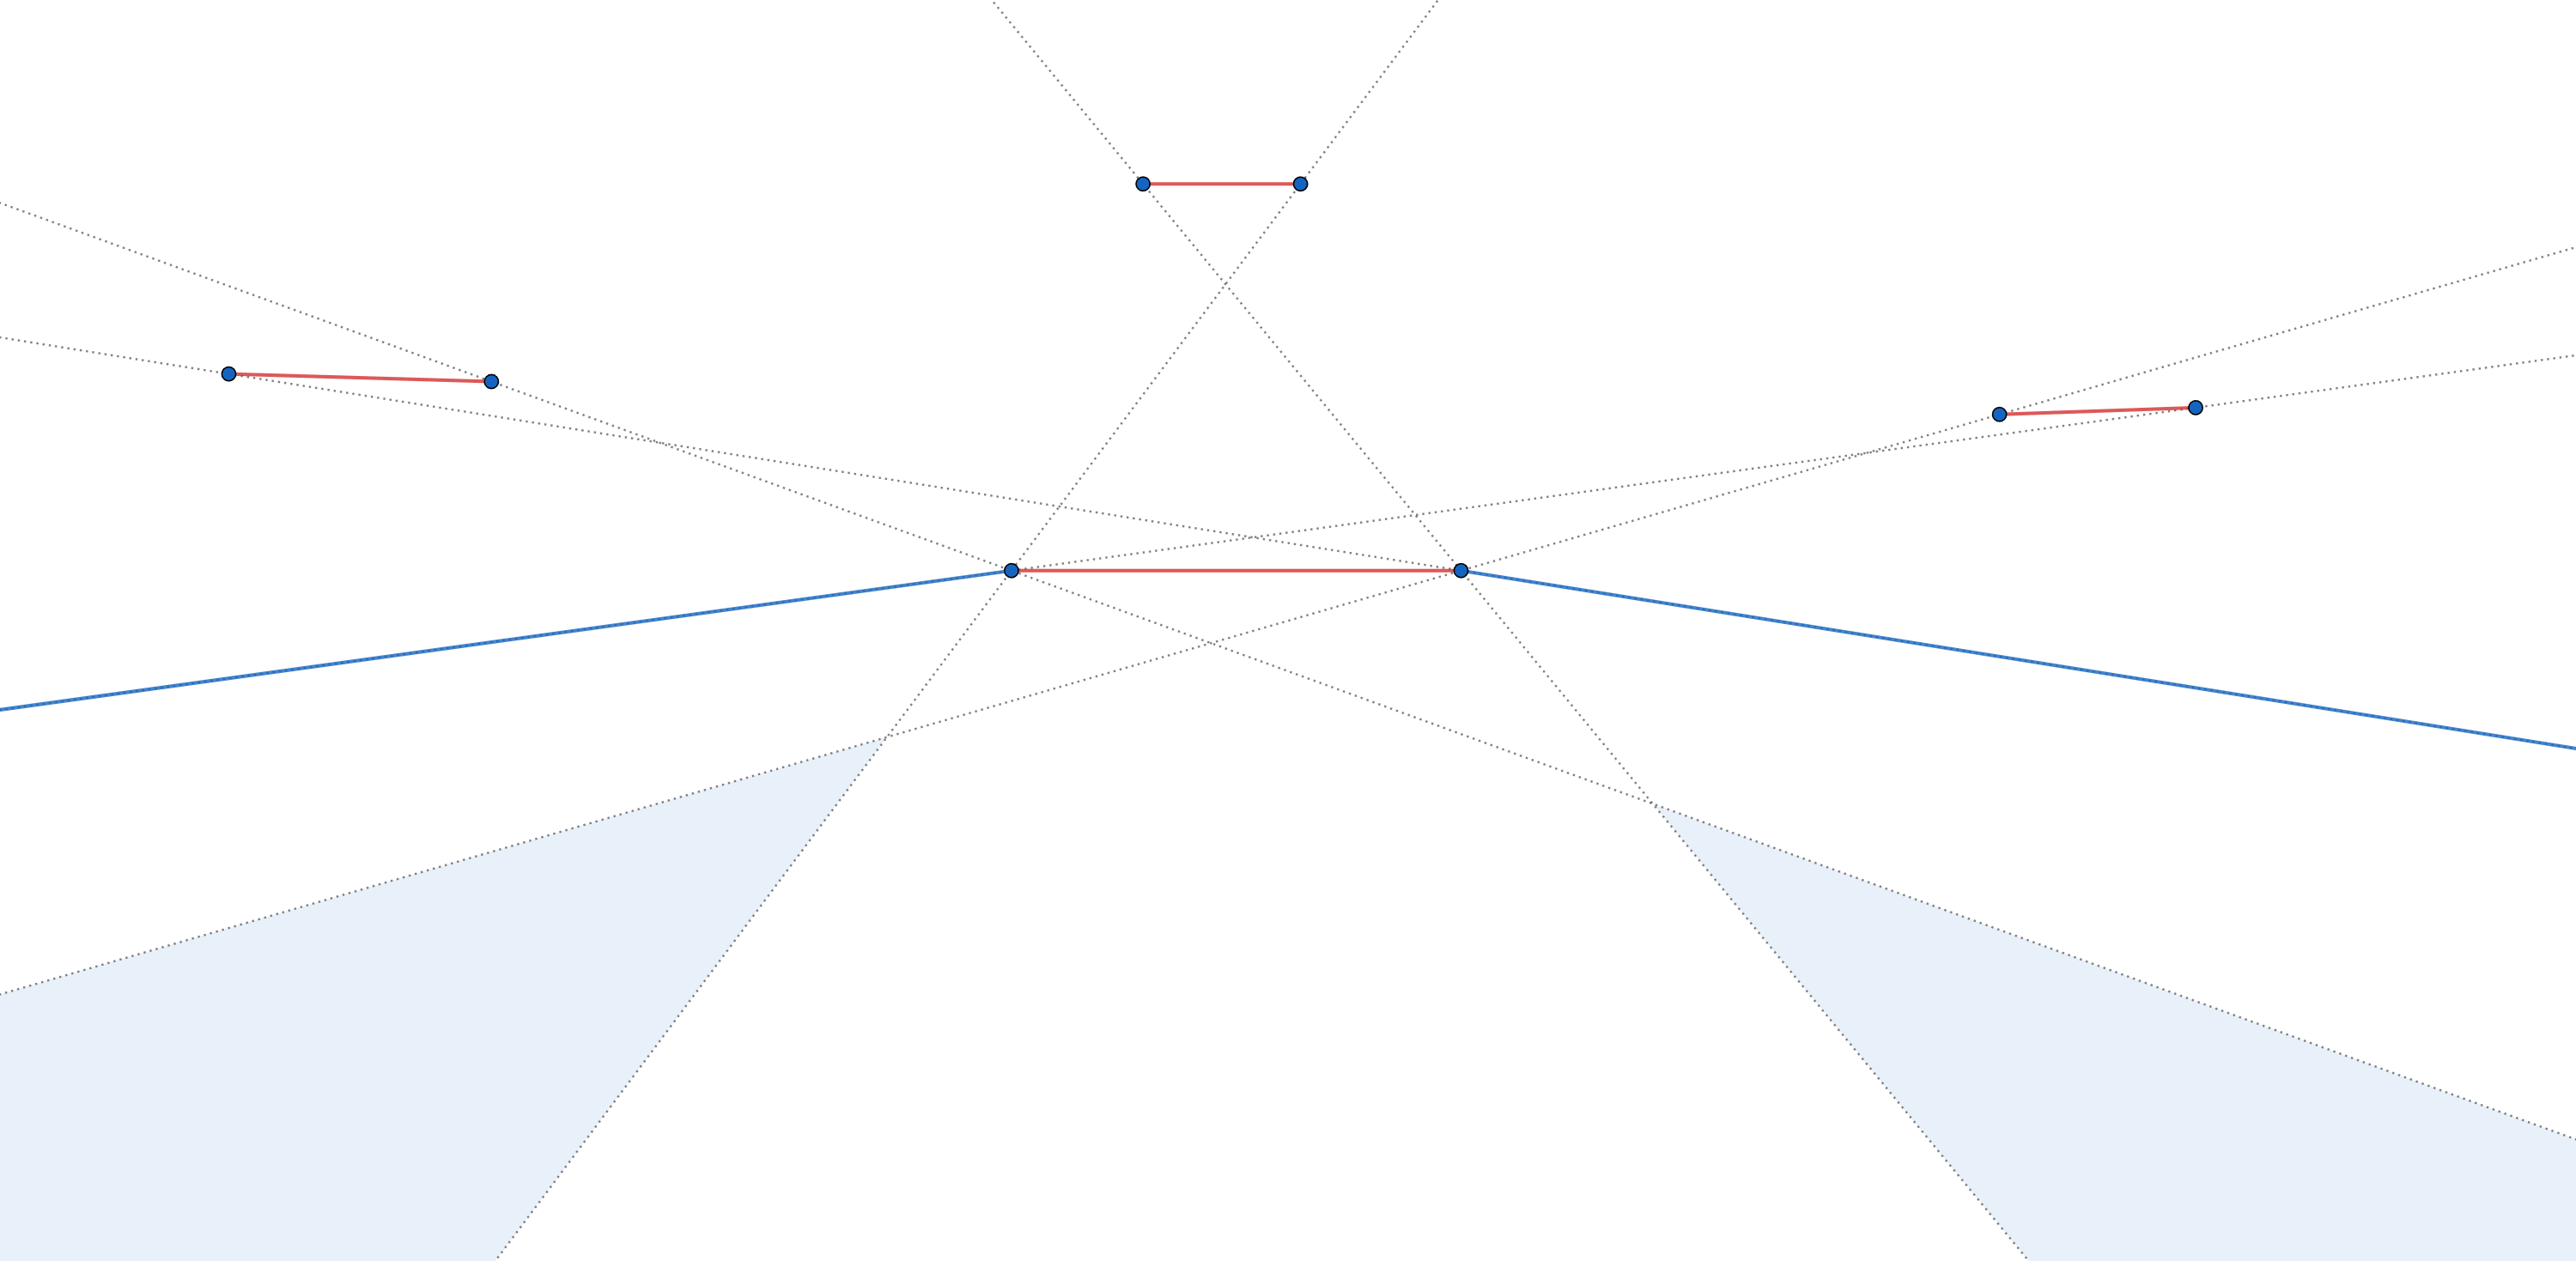
\includegraphics[width=0.5\linewidth]{no_zone_S1_hard.png}
\end{figure}

Для нахождения данной облаcти можно построить arrangment
на n участвующих в ее построение прямых и перебрать грани.
Сложность такого алгоритма $O(n^2)$. Однако сложность
вырезаемых клиньев константна, а значит и сложность зоны
лишь линейна, что дает надежду на существование более быстрого
алгоритма.

Аналогично для $S_2$.

Существование хотя бы одного отрезка в $S_3$ порождает
одну область <<нет-зоны>>, ограниченную двумя лучами.
Для ее построения достаточно найти такие  $q_1, q_2 \in P_3$,
которые бы минимизировали углы $q_1 p_1 p_2$, $q_2 p_1 p_2$
при условии того, что $q_1$ лежит левее $p_1 p_2$, а $q_1$
правее. Далее строятся прямые на $q_1 p_1$ и $q_2 p_1$. 
Искомые лучи лежат на полученных прямых, начинаются с 
$p_1$, не включают $q_1$ и $q_2$.
\begin{figure}[H]
      \centering
      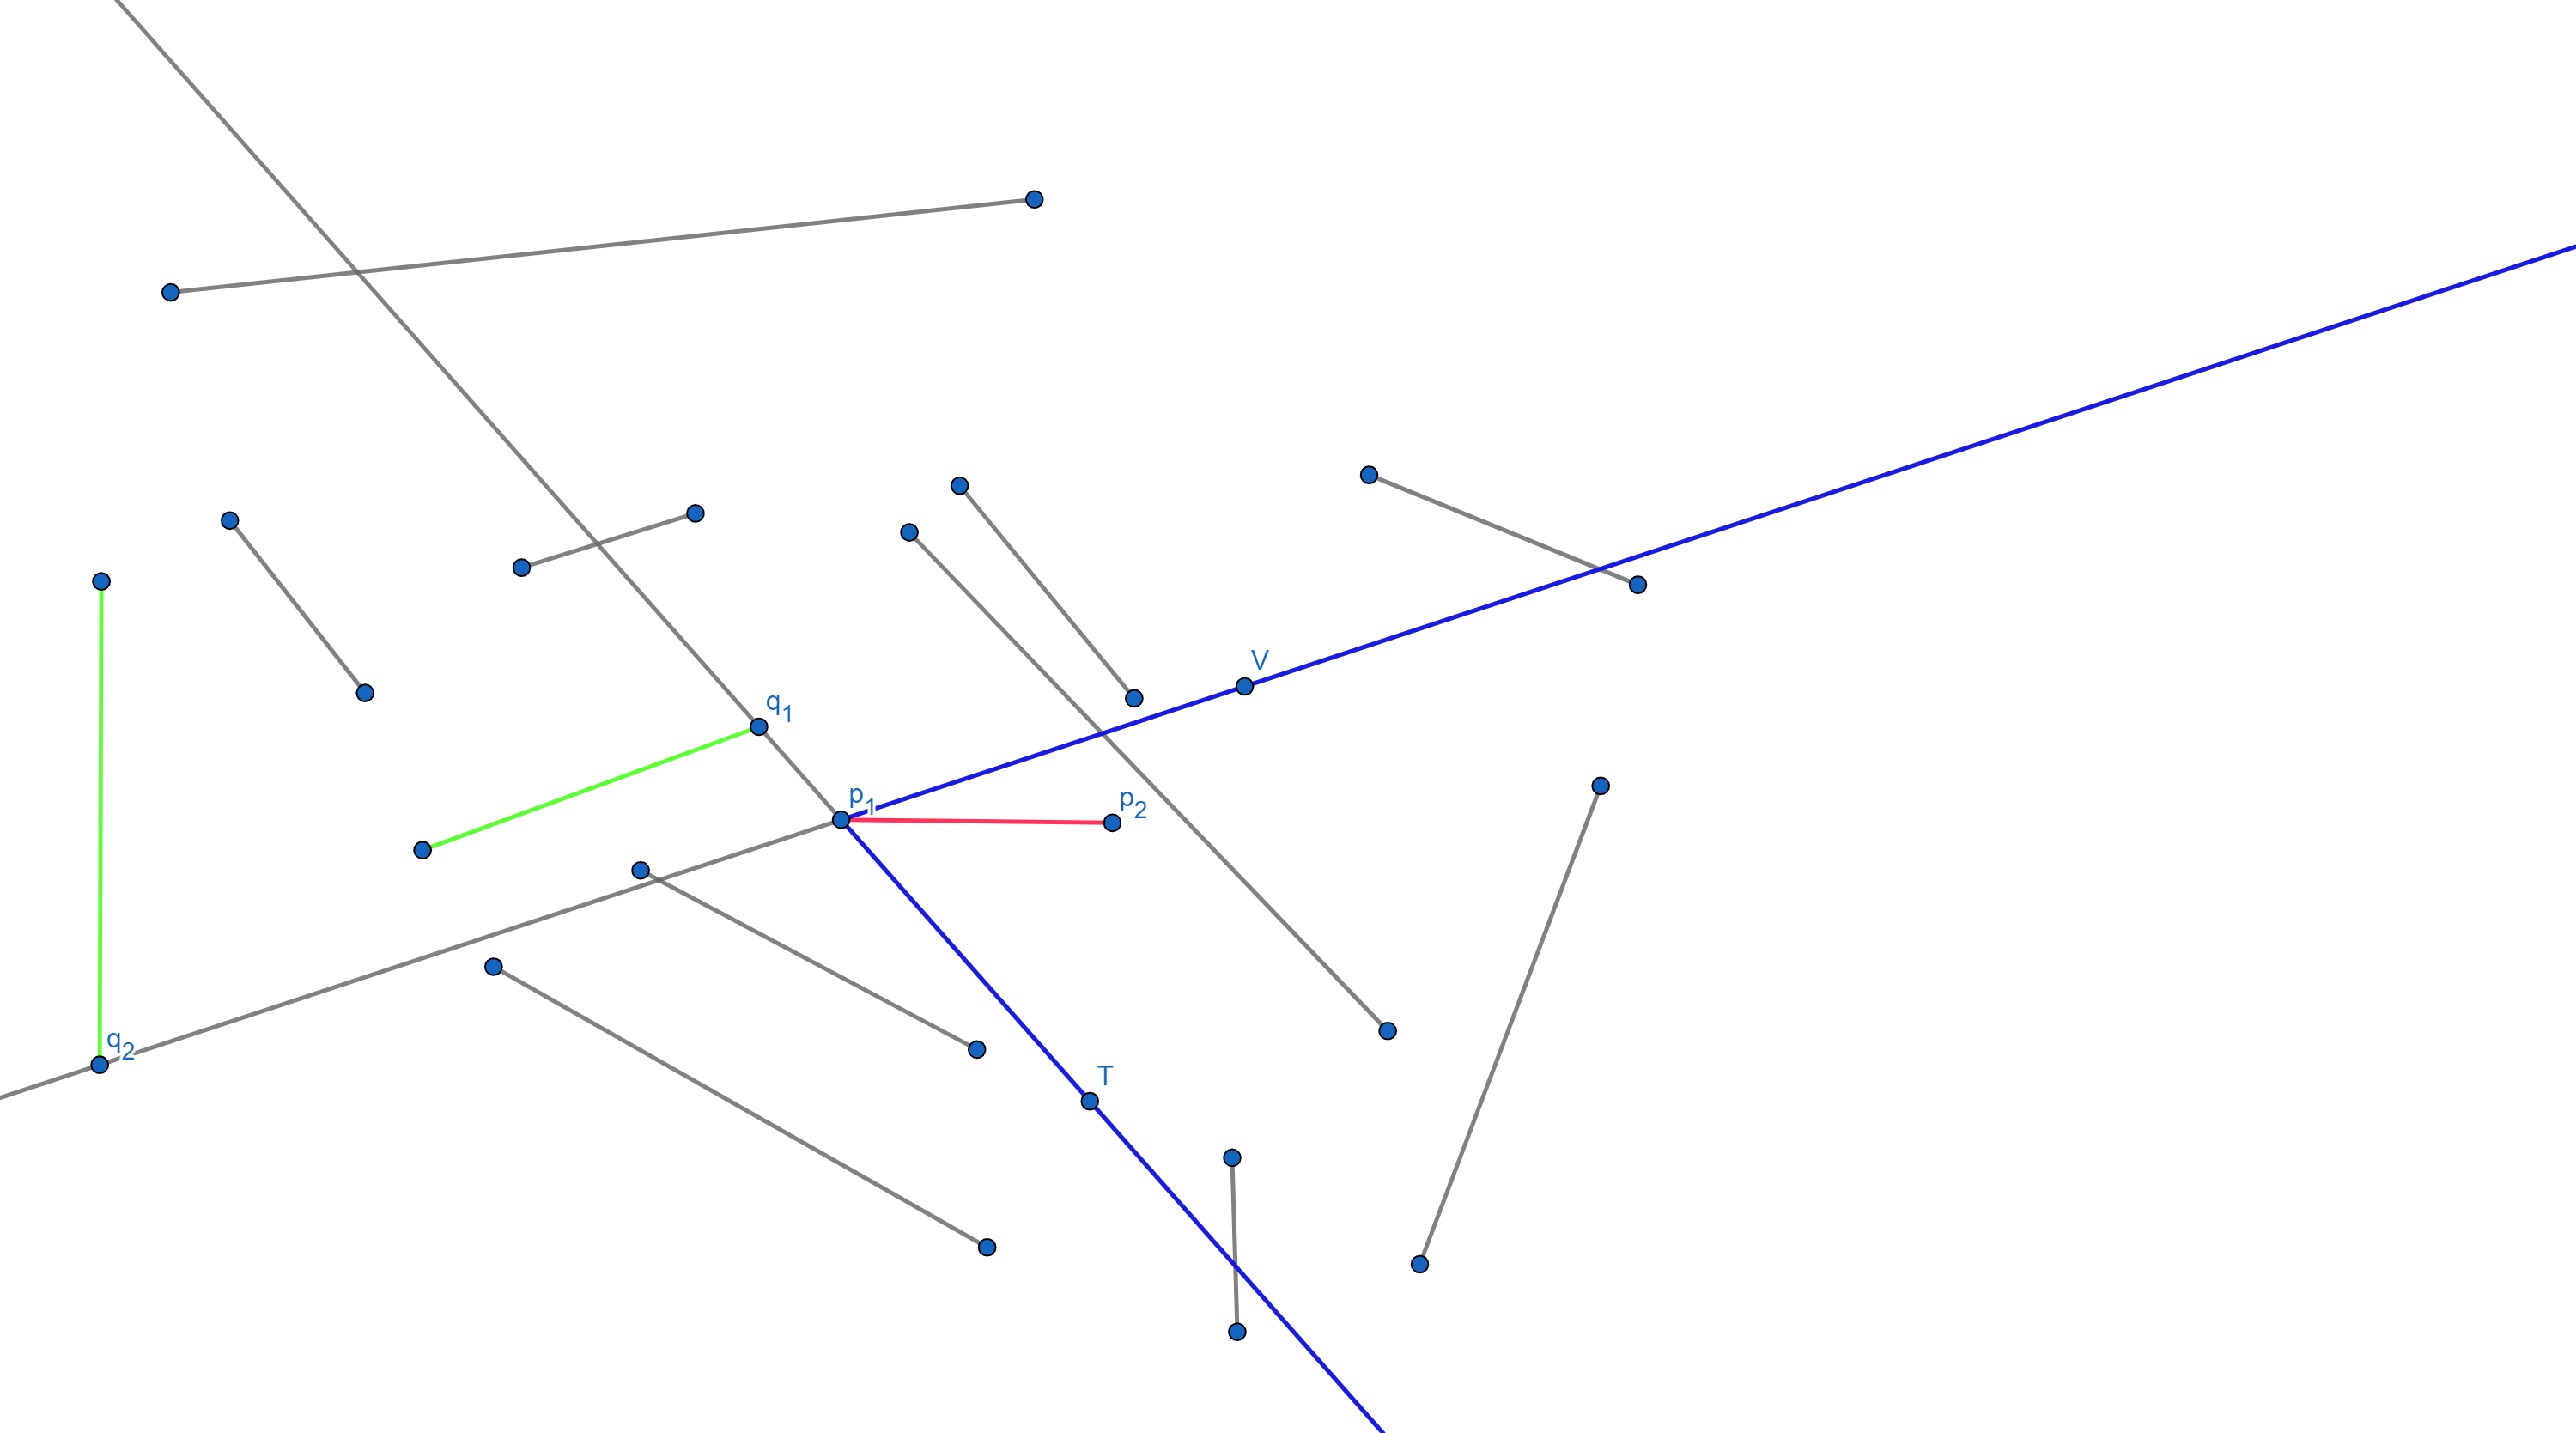
\includegraphics[width=0.5\linewidth]{rays_3.png}
\end{figure}

Для $S_4$ минимизируются углы $q_1 p_2 p_1$, $q_2 p_2 p_1$,
лучи начинаются с $p_2$.
\begin{figure}[H]
      \centering
      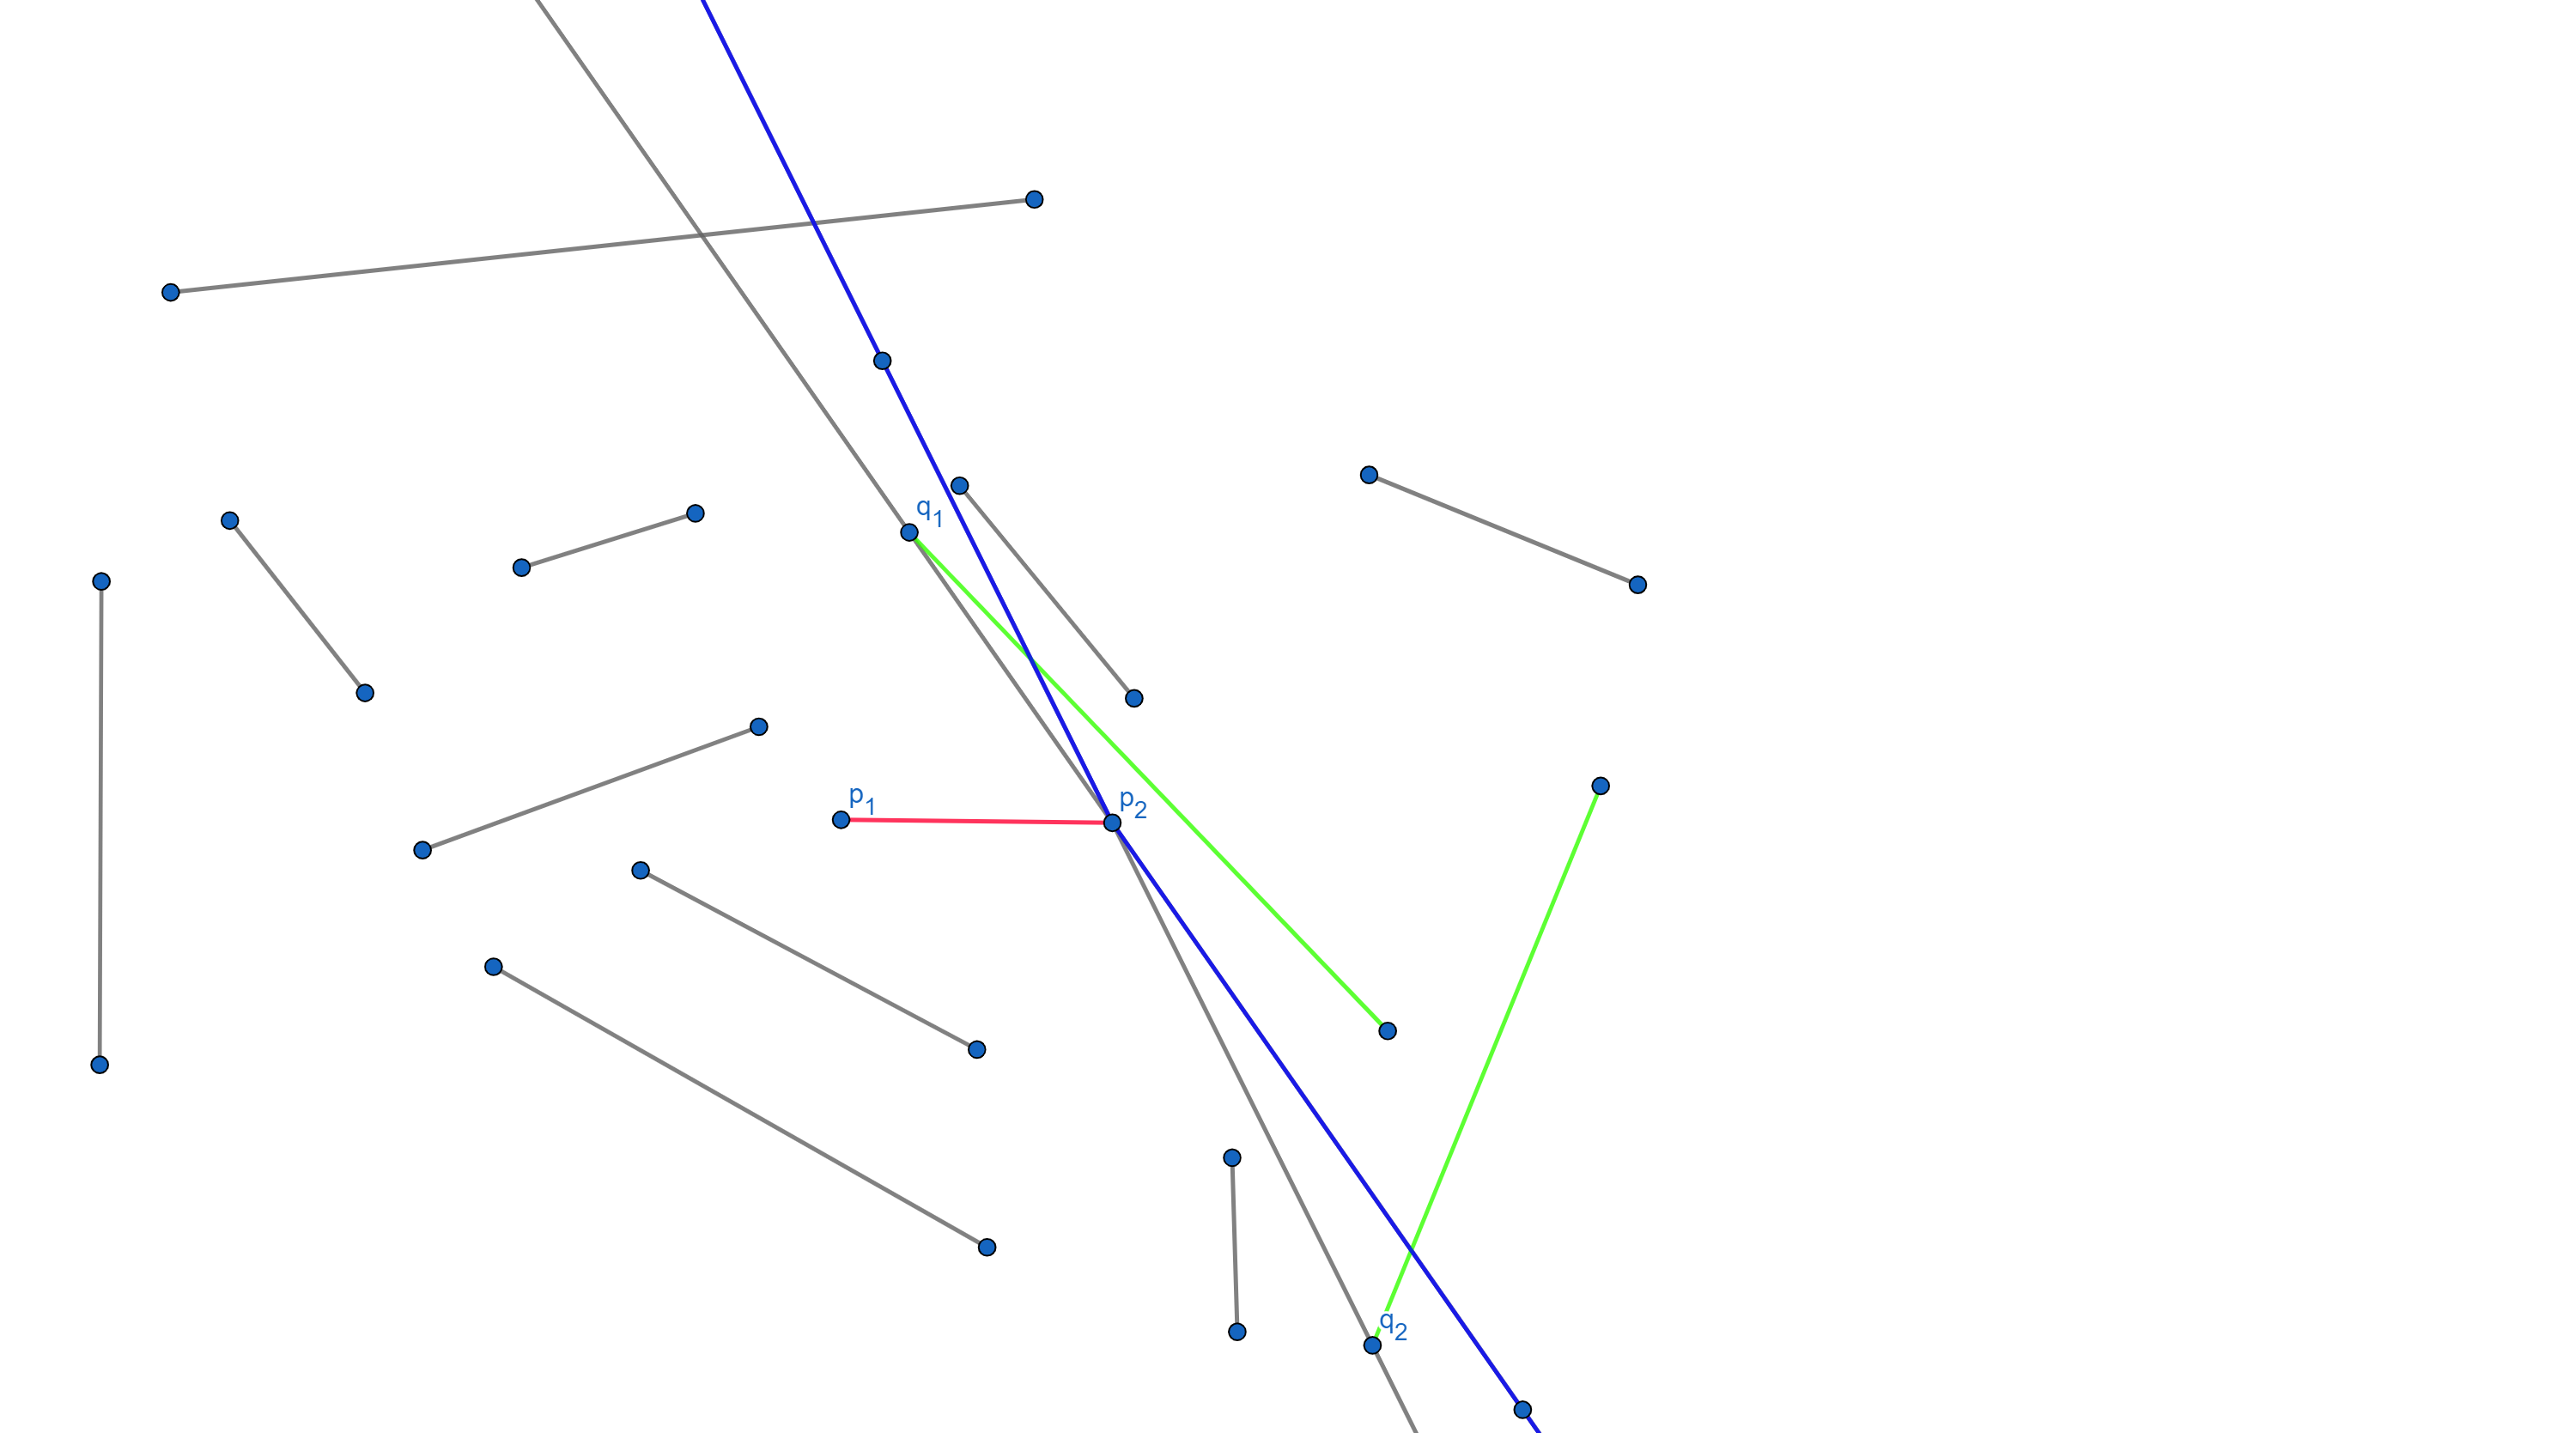
\includegraphics[width=0.5\linewidth]{rays_4.png}
\end{figure}

Перед следующим шагом необходимо пересечь все получившиеся
нет-зоны одного отрезка. Очевидно, что у нет-зон $S_1, S_2$
пересечение пусто. Так что данная операция сводится к пересечению
нет-зон $S_3, S_4$ с $S_1, S_2$ и друг-другом, делается за $O(n)$.

Для построения пересечения (поиска области являющейся
пересечением да-зон) на этапе построения нет-зон можно запомнить
для каждой прямой, какие лучи/отрезки каких нет-зон он порождает.
(обозначим кол-во объектов для каждой прямой за $k$. $k \leq 2$.)
После построения всех нет-зон, на всех прямых c $k \geq 1$
строится arrangment. В РСДС ищем грань, в которой все отрезки
никого не закрывают (пересечение да-зон). С учетом имеющихся
данных обход делается за $O(n^4)$.

\end{document}